\chapter{Eksploratorna analiza}

\section{Opis atributa}
\begin{table}[h]
	\centering
	\begin{tabular}{|c|c|p{8cm}|}
	\hline
	\textbf{Atribut} & \textbf{Tip podatka} & \textbf{Opis} \\ \hline
	track\_id & character & Jedinstveni ID pjesme \\ \hline
	track\_name & character & Naziv pjesme \\ \hline
	track\_artist & character & Izvođač pjesme \\ \hline
	track\_popularity & double & Popularnost pjesme (0-100) \\ \hline
	track\_album\_id & character & Jedinstveni ID albuma \\ \hline
	track\_album\_name & character & Naziv albuma na kojem se nalazi pjesma \\ \hline
	track\_album\_release\_date & character & Datum izlaska albuma \\ \hline
	playlist\_name & character & Naziv playliste \\ \hline
	playlist\_id & character & Jedinstveni ID playliste \\ \hline
	playlist\_genre & character & Žanr playliste \\ \hline
	playlist\_subgenre & character & Podžanr playliste \\ \hline
	danceability & double & Plesnost (koliko je pjesma prikladna za plesanje u rasponu 0.0-1.0) \\ \hline
	energy & double & Energičnost (perceptualna mjera intenziteta i aktivnosti u rasponu 0.0-1.0) \\ \hline
	key & double & Ukupni tonalitet pjesme \\ \hline
	loudness & double & Glasnoća pjesme u decibelima \\ \hline
	mode & double & Modus pjesme (1 - veliki, 0 - mali) \\ \hline
	speechiness & double & Prisutnost izgovorenih riječi u pjesmi \\ \hline
	acousticness & double & Mjera povjerenja je li pjesma akustična u rasponu od 0.0 do 1.0 \\ \hline
	instrumentalness & double & Sadrži li pjesma vokale \\ \hline
	liveness & double & Detektira prisutnost publike u snimci \\ \hline
	valence & double & Mjera od 0.0 do 1.0 koja opisuje glazbenu pozitivnost koju prijenosi pjesma \\ \hline
	tempo & double & Ukupno procijenjeni tempo pjesme u udarcima po minuti (BPM) \\ \hline
	duration\_ms & double & Trajanje pjesme u milisekundama \\ \hline
	\end{tabular}
	\caption{Opis tablice podataka o glazbi}
	\label{tab:glazba}
	\end{table}

\clearpage
\section{Proces učitavanja i prilagodbe podataka}

	\subsubsection{Proces učitavanja podataka}
	
		\textbf{Učitavanje podataka:}
		\begin{figure}[H]
			\centering
			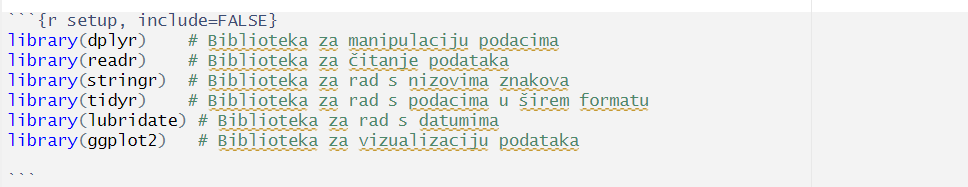
\includegraphics[scale=0.7]{slike/ucitavanje.png}
			% Veličina slike u odnosu na originalnu datoteku i pozicija slike
			\caption{\textbf{Korištene biblioteke \textit{}}}
		\end{figure}
		\begin{figure}[H]
			\centering
			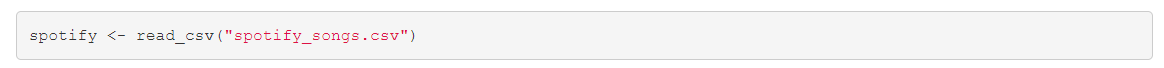
\includegraphics[scale=0.7]{slike/spotify.png}
			% Veličina slike u odnosu na originalnu datoteku i pozicija slike
			\caption{\textbf{Učitavanje podatkovnog okvira \textit{spotify\_songs}}}
		\end{figure}
		
		\begin{figure}[H]
			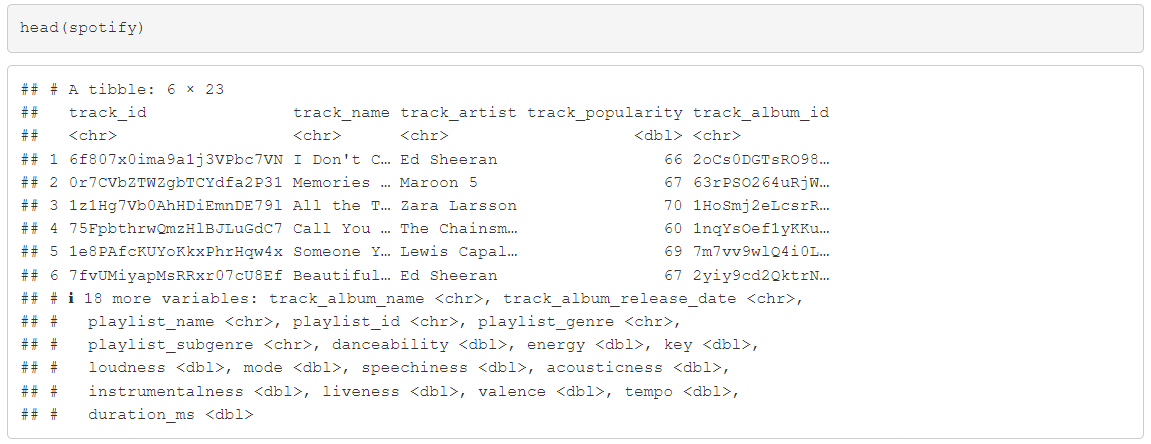
\includegraphics[scale=0.7]{slike/head.png}
			\centering
			\caption{Rezultat poziva \textit{head} funckije}
			
		\end{figure}
		
		\begin{figure}[H]
			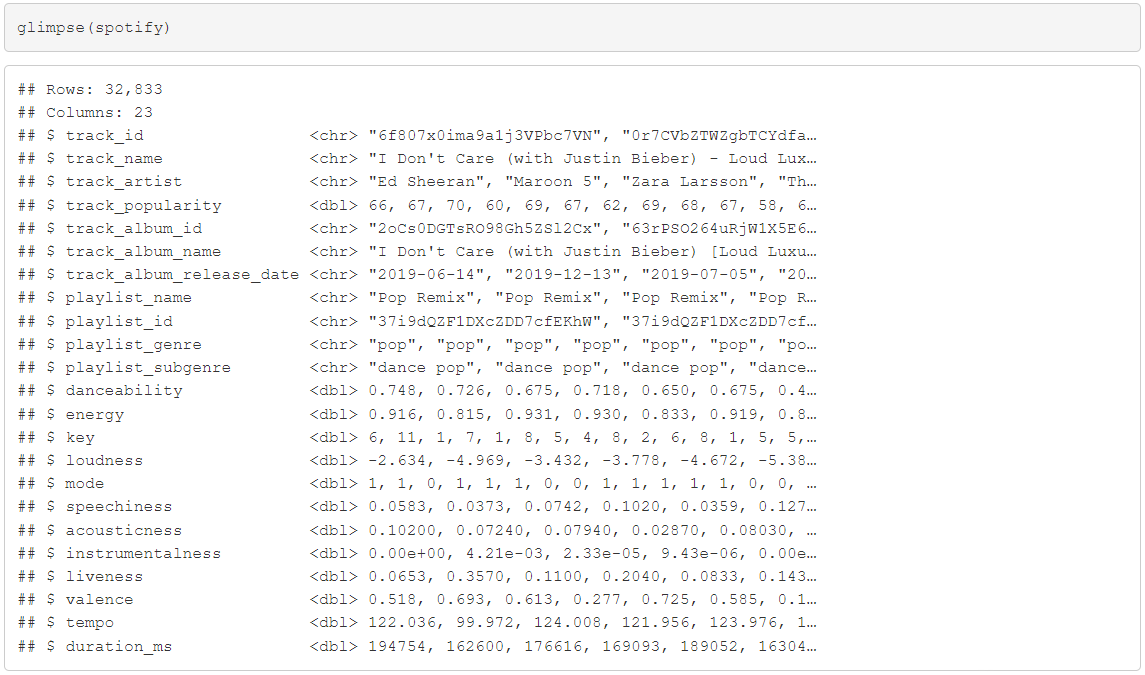
\includegraphics[scale=0.7]{slike/glimpse.png}
			\centering
			\caption{Rezultat poziva \textit{glimpse} funckije}
			
		\end{figure}
		
		\begin{figure}[H]
			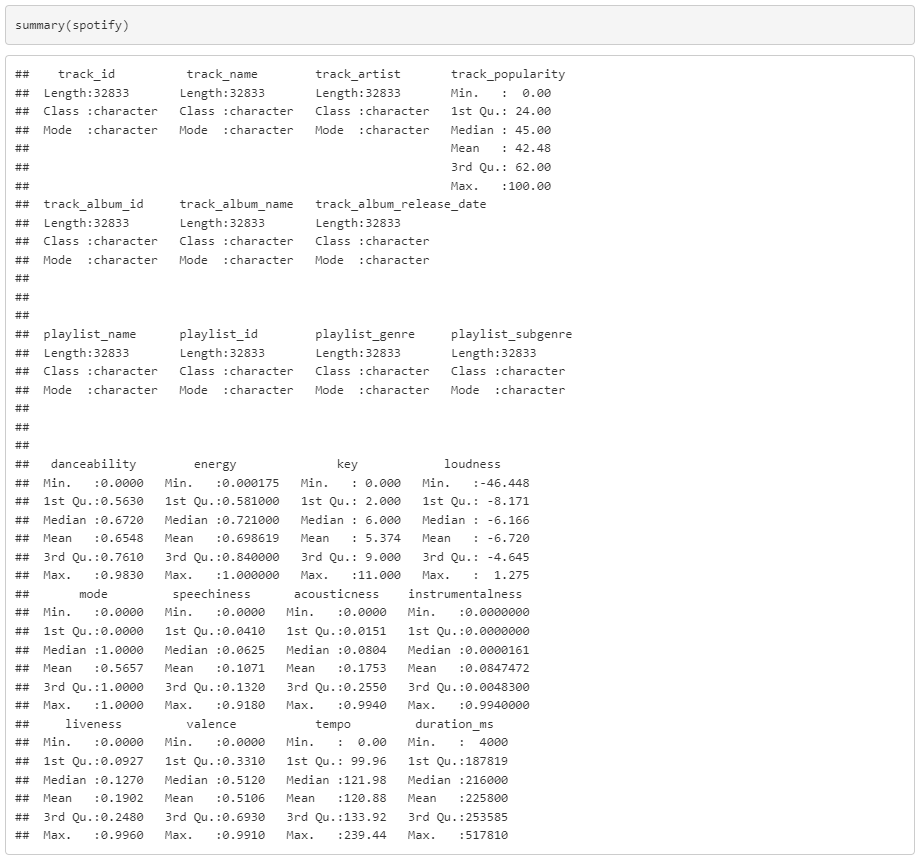
\includegraphics[scale=0.7]{slike/summary.png}
			\centering
			\caption{Rezultat poziva \textit{summary} funckije}
			
		\end{figure}
		
		U prikazanim kodovima sa slika, koristimo različite R pakete kako bismo pripremili i istražili skup podataka "spotify\_songs.csv". Prvo, koristimo pakete poput \textbf{readr}, \textbf{dplyr} i \textbf{stringr} za čitanje i manipulaciju podacima. Nakon toga, prikazujemo prvih nekoliko redova podataka pomoću funkcije \textbf{head} kako bismo dobili inicijalni uvid u strukturu podataka.
		
		Zatim, koristimo funkciju \textbf{glimpse} za detaljniji pregled strukture podataka, prikazujući informacije o varijablama, njihovim tipovima podataka i prvim redovima podataka. Na kraju, koristimo funkciju \textbf{summary} kako bismo dobili osnovne statističke informacije o numeričkim varijablama u skupu podataka.
		
		Ovi koraci omogućuju nam osnovni uvid u strukturu podataka prije nego što nastavimo s daljnjom analizom i vizualizacijom.
		
	
	\subsubsection{Proces prilagodbe podataka}
	Stupce \textit{playlist\_genre} te \textit{playlist\_subgenre} pretvorili smo u u faktore s obzirom da postoji određen broj kategorija jedne i druge varijable. U podatkovnom okviru također postoji 5 redaka s null vrijednostima, koji su izbačeni radi lakšeg rada s grafovima.
	
	\begin{figure}[H]
		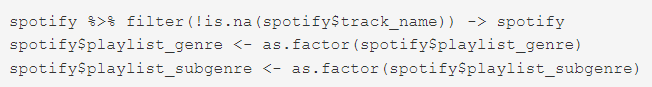
\includegraphics[scale=0.9]{slike/prilagodba.png}
		\centering
		\caption{Prilagodba podataka}
		
	\end{figure}
	


\clearpage
\section{Vizualizacija Podataka}
	Vizualizacija podataka postaje ključna komponenta analize i interpretacije kompleksnih skupova podataka. 
	U ovom podpoglavlju istražujemo moć vizualizacije u kontekstu glazbene platforme Spotify, prezentirajući neke od grafova kako bismo bolje razumjeli glazbene obrasce, preferencije slušatelja te dinamiku glazbene industrije.
	
	\subsubsection{1) Histogram popularnosti pjesama}
	
	\textbf{Opis grafa:}
	
	Ovaj graf prikazuje histogram popularnosti. Prikazuje distribuciju popularnosti pjesama. Na x-osi nalaze se razine popularnosti pjesama, a y-osi broj pjesama koje se nalaze u pojedinoj razini popularnosti.
	Ovaj histogram omogućava vizualni pregled koje su razine popularnosti češće, a koje rjeđe. 
	Iz grafa je očigledno da je većina pjesama nepopularna u ovom skupu podataka, što je logično s obzirom na veliki broj dostupnih pjesama.

	\textbf{Slika grafa:}
	\begin{figure}[H]
		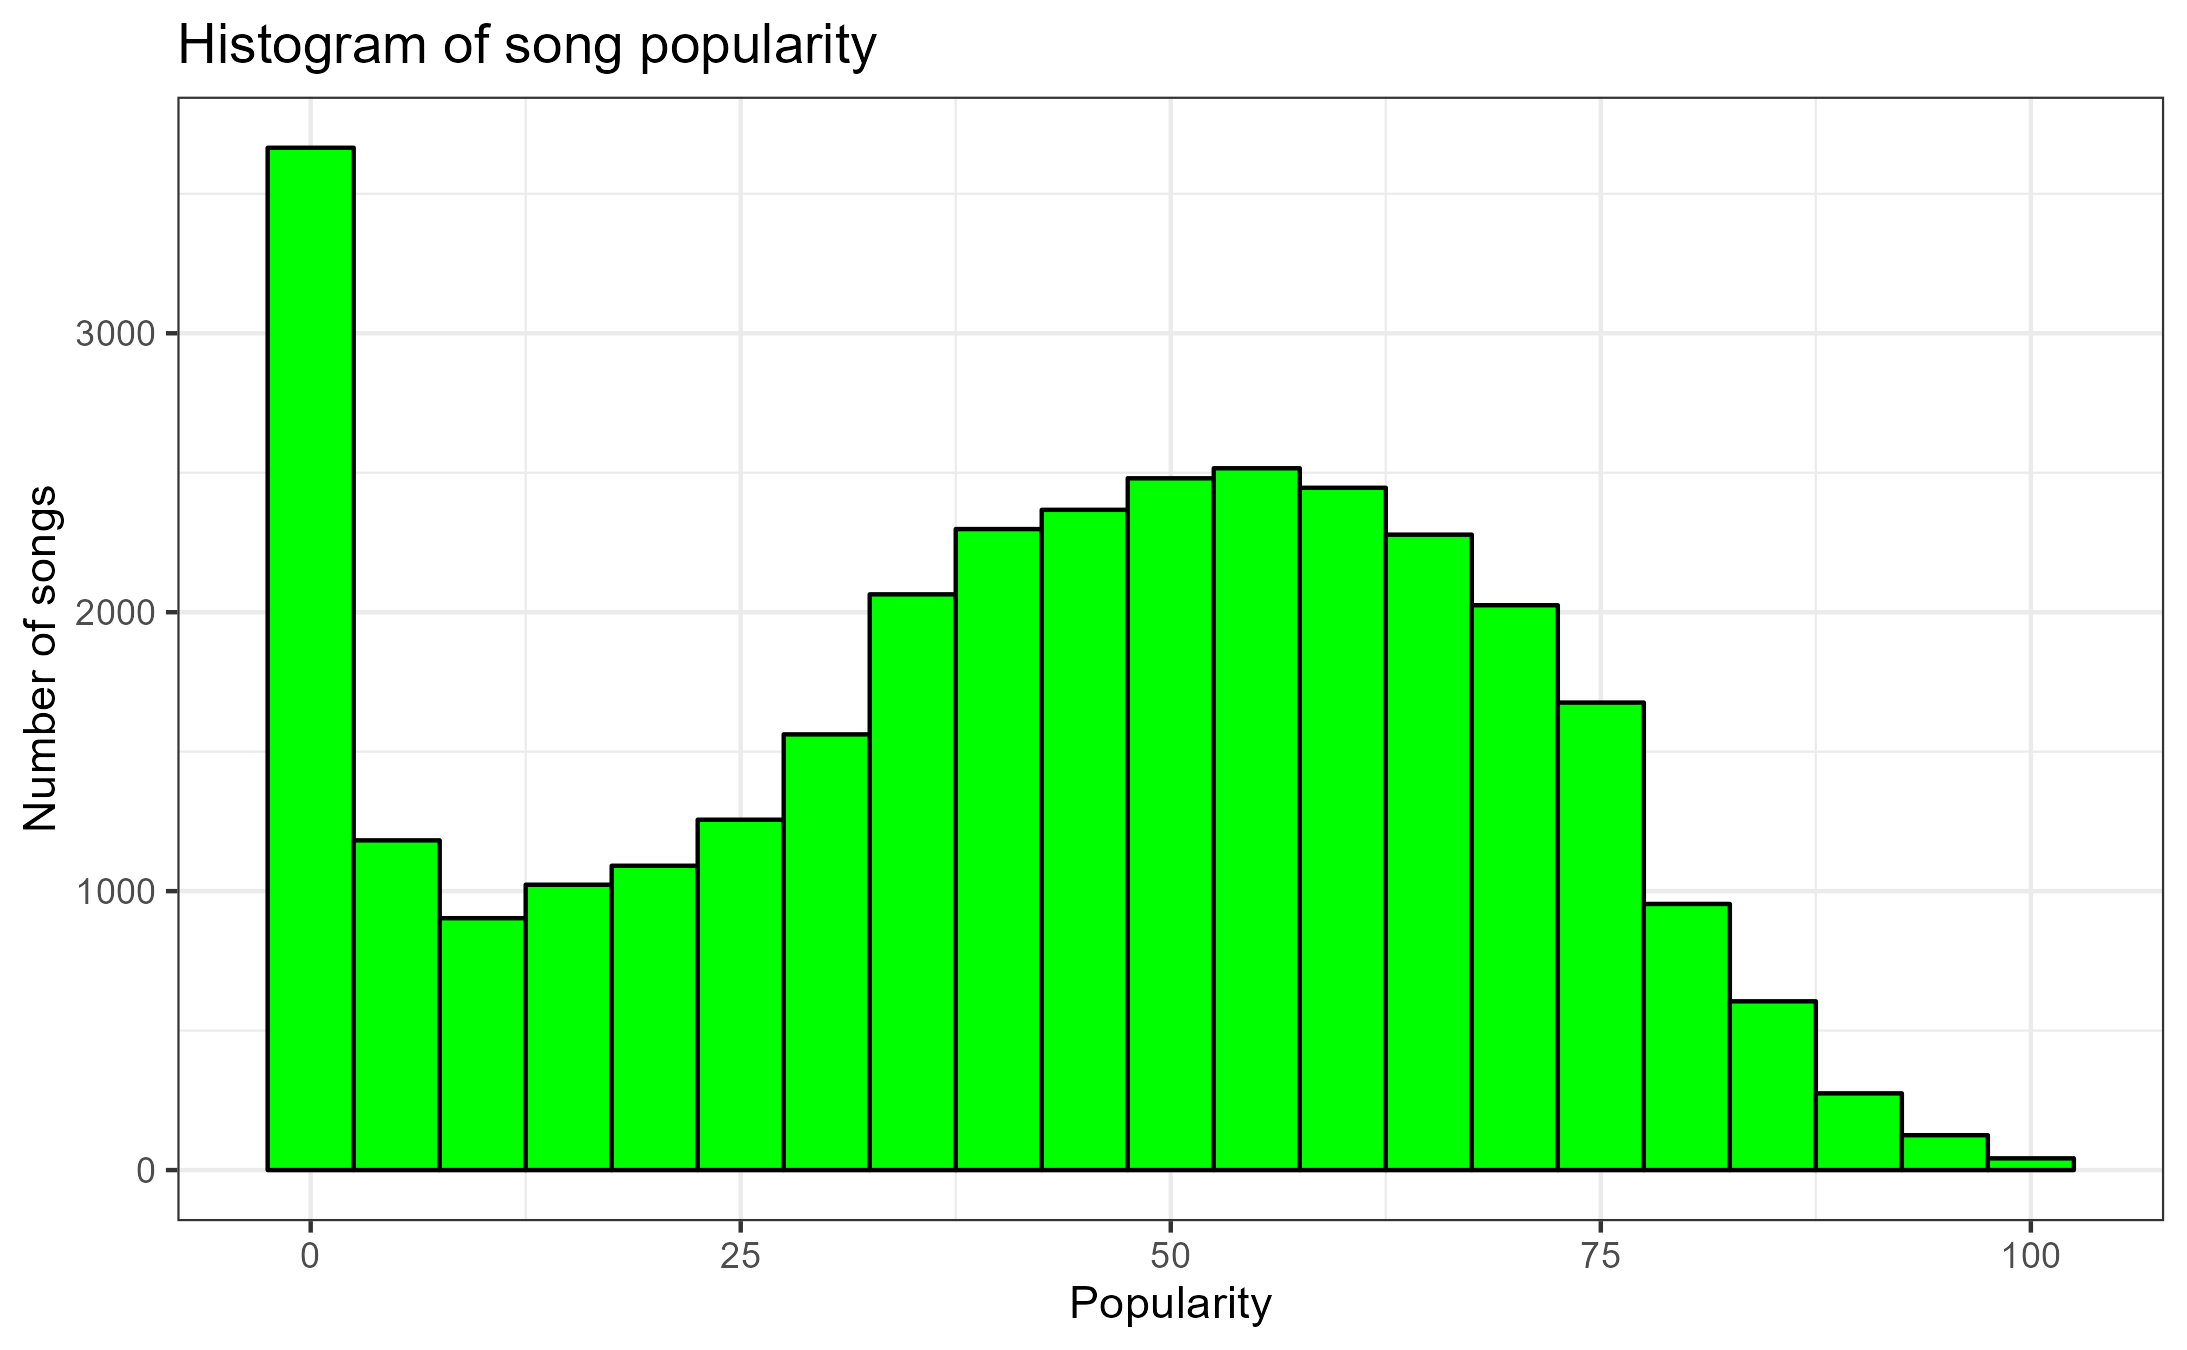
\includegraphics[scale=0.9]{slike/Histogram of song popularity.png}
		%veličina slike u odnosu na originalnu datoteku i pozicija slike
		\centering
		\caption{Histogram popularnosti pjesama}
		
	\end{figure}

	\subsubsection{2) Top 10 umjetnika po popularnosti}
	
	\textbf{Opis grafa:}
	
	Ovaj graf prikazuje deset najpopularnijih glazbenih izvođača temeljem prosječne popularnosti njihovih pjesama. Izračunata je srednja vrijednost popularnosti za svakog izvođača, a zatim su odabrani najbolji deset izvođača prema toj mjeri popularnosti.
	Na x-osi su navedeni izvođači, poredani prema visini prosječne popularnosti, dok y-os prikazuje prosječnu popularnost. Svaki šareni stupac predstavlja jednog izvođača, a visina stupa označava njegovu prosječnu popularnost.
	Ovaj graf pruža brz i pregledan način usporedbe popularnosti izvođača, omogućujući identifikaciju najboljih deset temeljem prosjeka popularnosti njihovih pjesama.
	
	\textbf{Slika grafa:}
	\begin{figure}[H]
		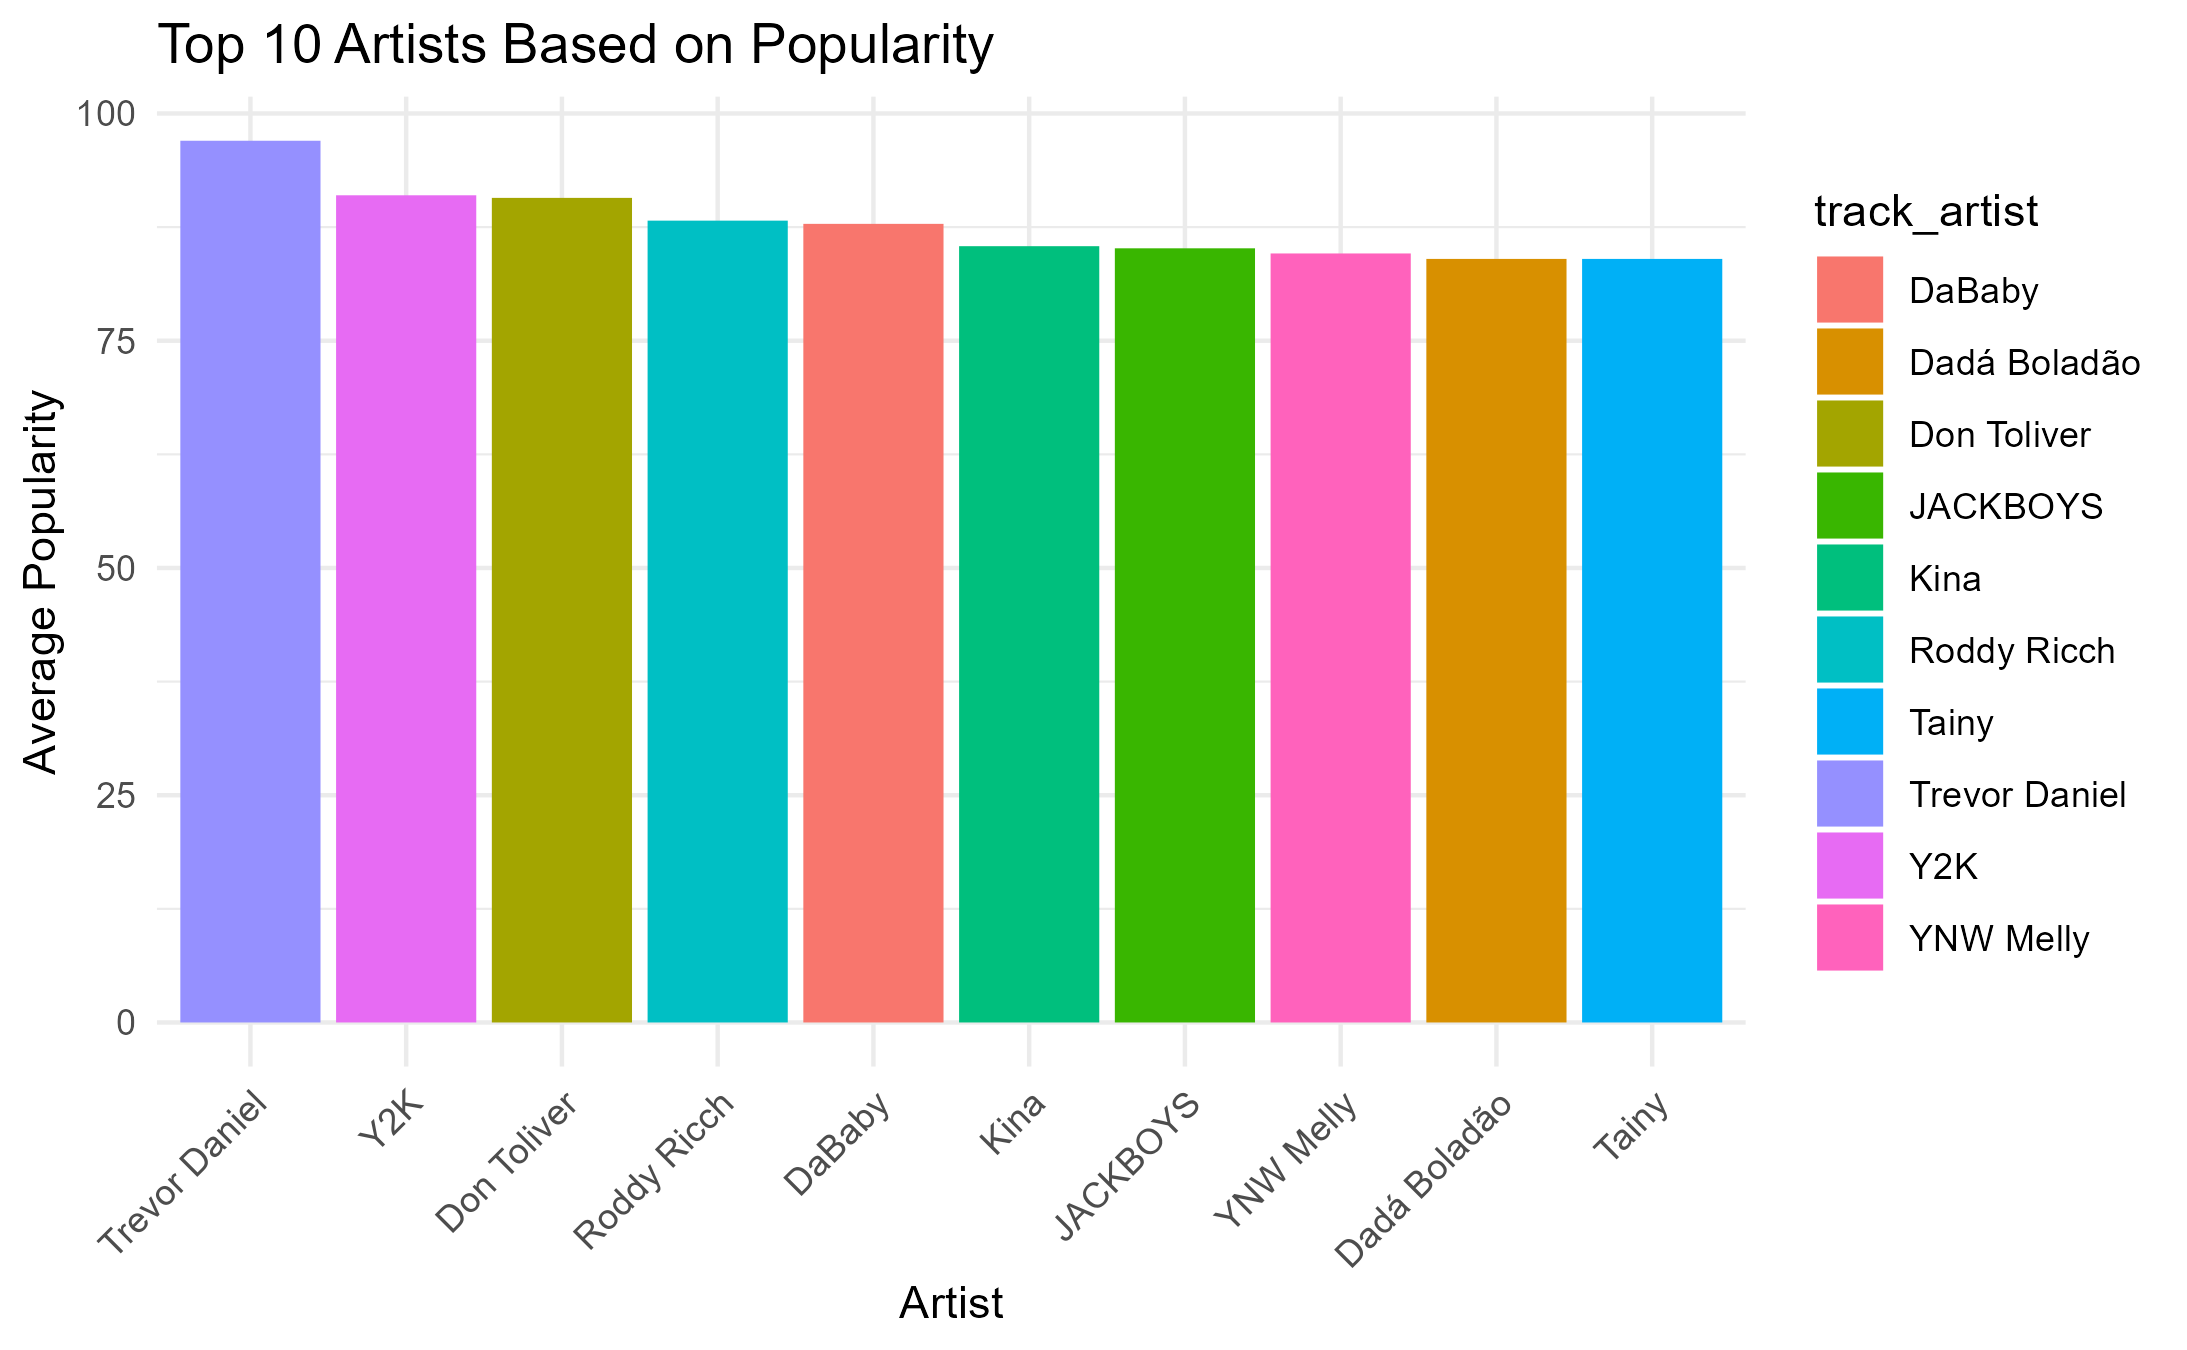
\includegraphics[scale=0.9]{slike/Top 10 popularity}
		%veličina slike u odnosu na originalnu datoteku i pozicija slike
		\centering
		\caption{Top 10 umjetnika po popularnosti}
		
	\end{figure}


	\subsubsection{3) Prosječna popularnost pjesama po godinama}
	
	\textbf{Opis grafa:}
	
	Ovaj stupčasti graf prikazuje prosječnu popularnost pjesama po godinama u razdoblju od 2000. godine do 2020. godine. X-os ovog grafa su godine u navedenom razdoblju (svaki stupac predstavlja jednu godinu), dok y-os predstavlja prosječnu popularnost. 
	Uvidom u ovaj graf možemo jednostavno vidjeti u kojoj su godini pjesme imale najveću popularnost, te vidjeti kako se popularnost mijenjala tokom tih 20 godina.
	S grafa je vidljivo da su najpopularnije pjesme izbačene 2019. godine.

	
	\textbf{Slika grafa:}
	\begin{figure}[H]
		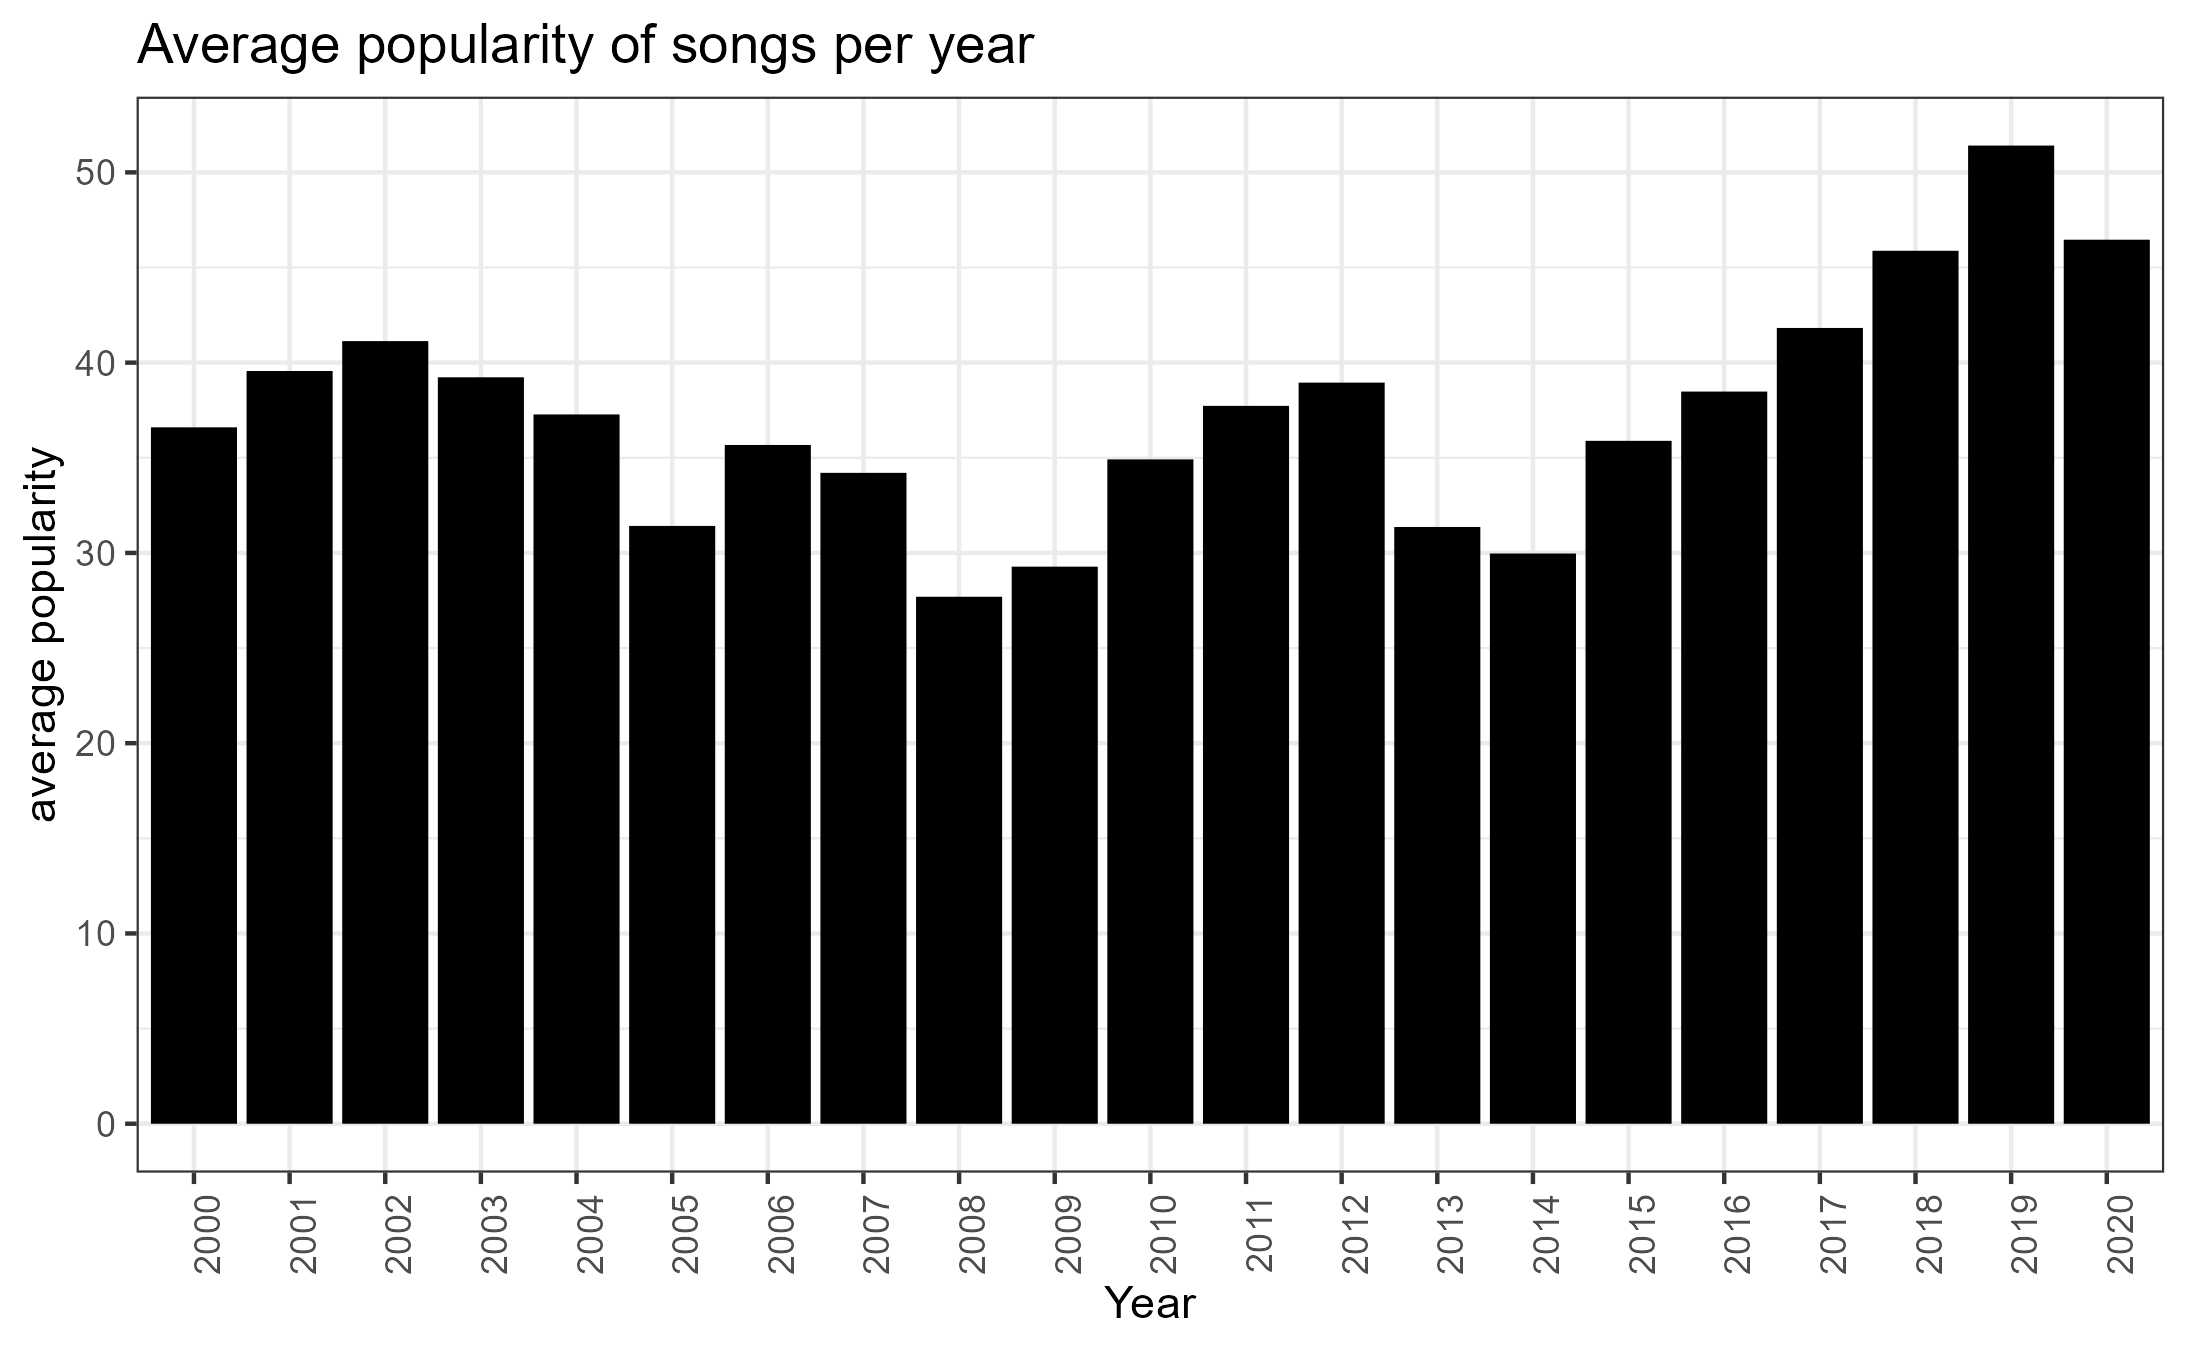
\includegraphics[scale=0.9]{slike/Average popularity of songs per year.png}
		%veličina slike u odnosu na originalnu datoteku i pozicija slike
		\centering
		\caption{Prosječna popularnost pjesama po godinama}
		
	\end{figure}
	
		\subsubsection{4) Distribucija energije kroz žanrove playlista}
	
	\textbf{Opis grafa:}
	
	Ovaj graf prikazuje distribuciju energije (y-os) na temelju različitih žanrova playlista (x-os). Svaki boxplot predstavlja jedan žanr, a njegova visina odražava raspon energije unutar tog žanra. Unutar svakog boxplota nalazi se pravokutnik koji predstavlja interkvartilni raspon, a linija unutar pravokutnika označava medijan energije
	Dodatno, postojanje "notcha" u sredini svakog boxplota pruža informaciju o razlikama u medijanima između žanrova.
	Iz ovog grafa se jasno može uočiti da su EDM i rock žanrovi najenergičniji.
	
		\textbf{Slika grafa:}
	\begin{figure}[H]
		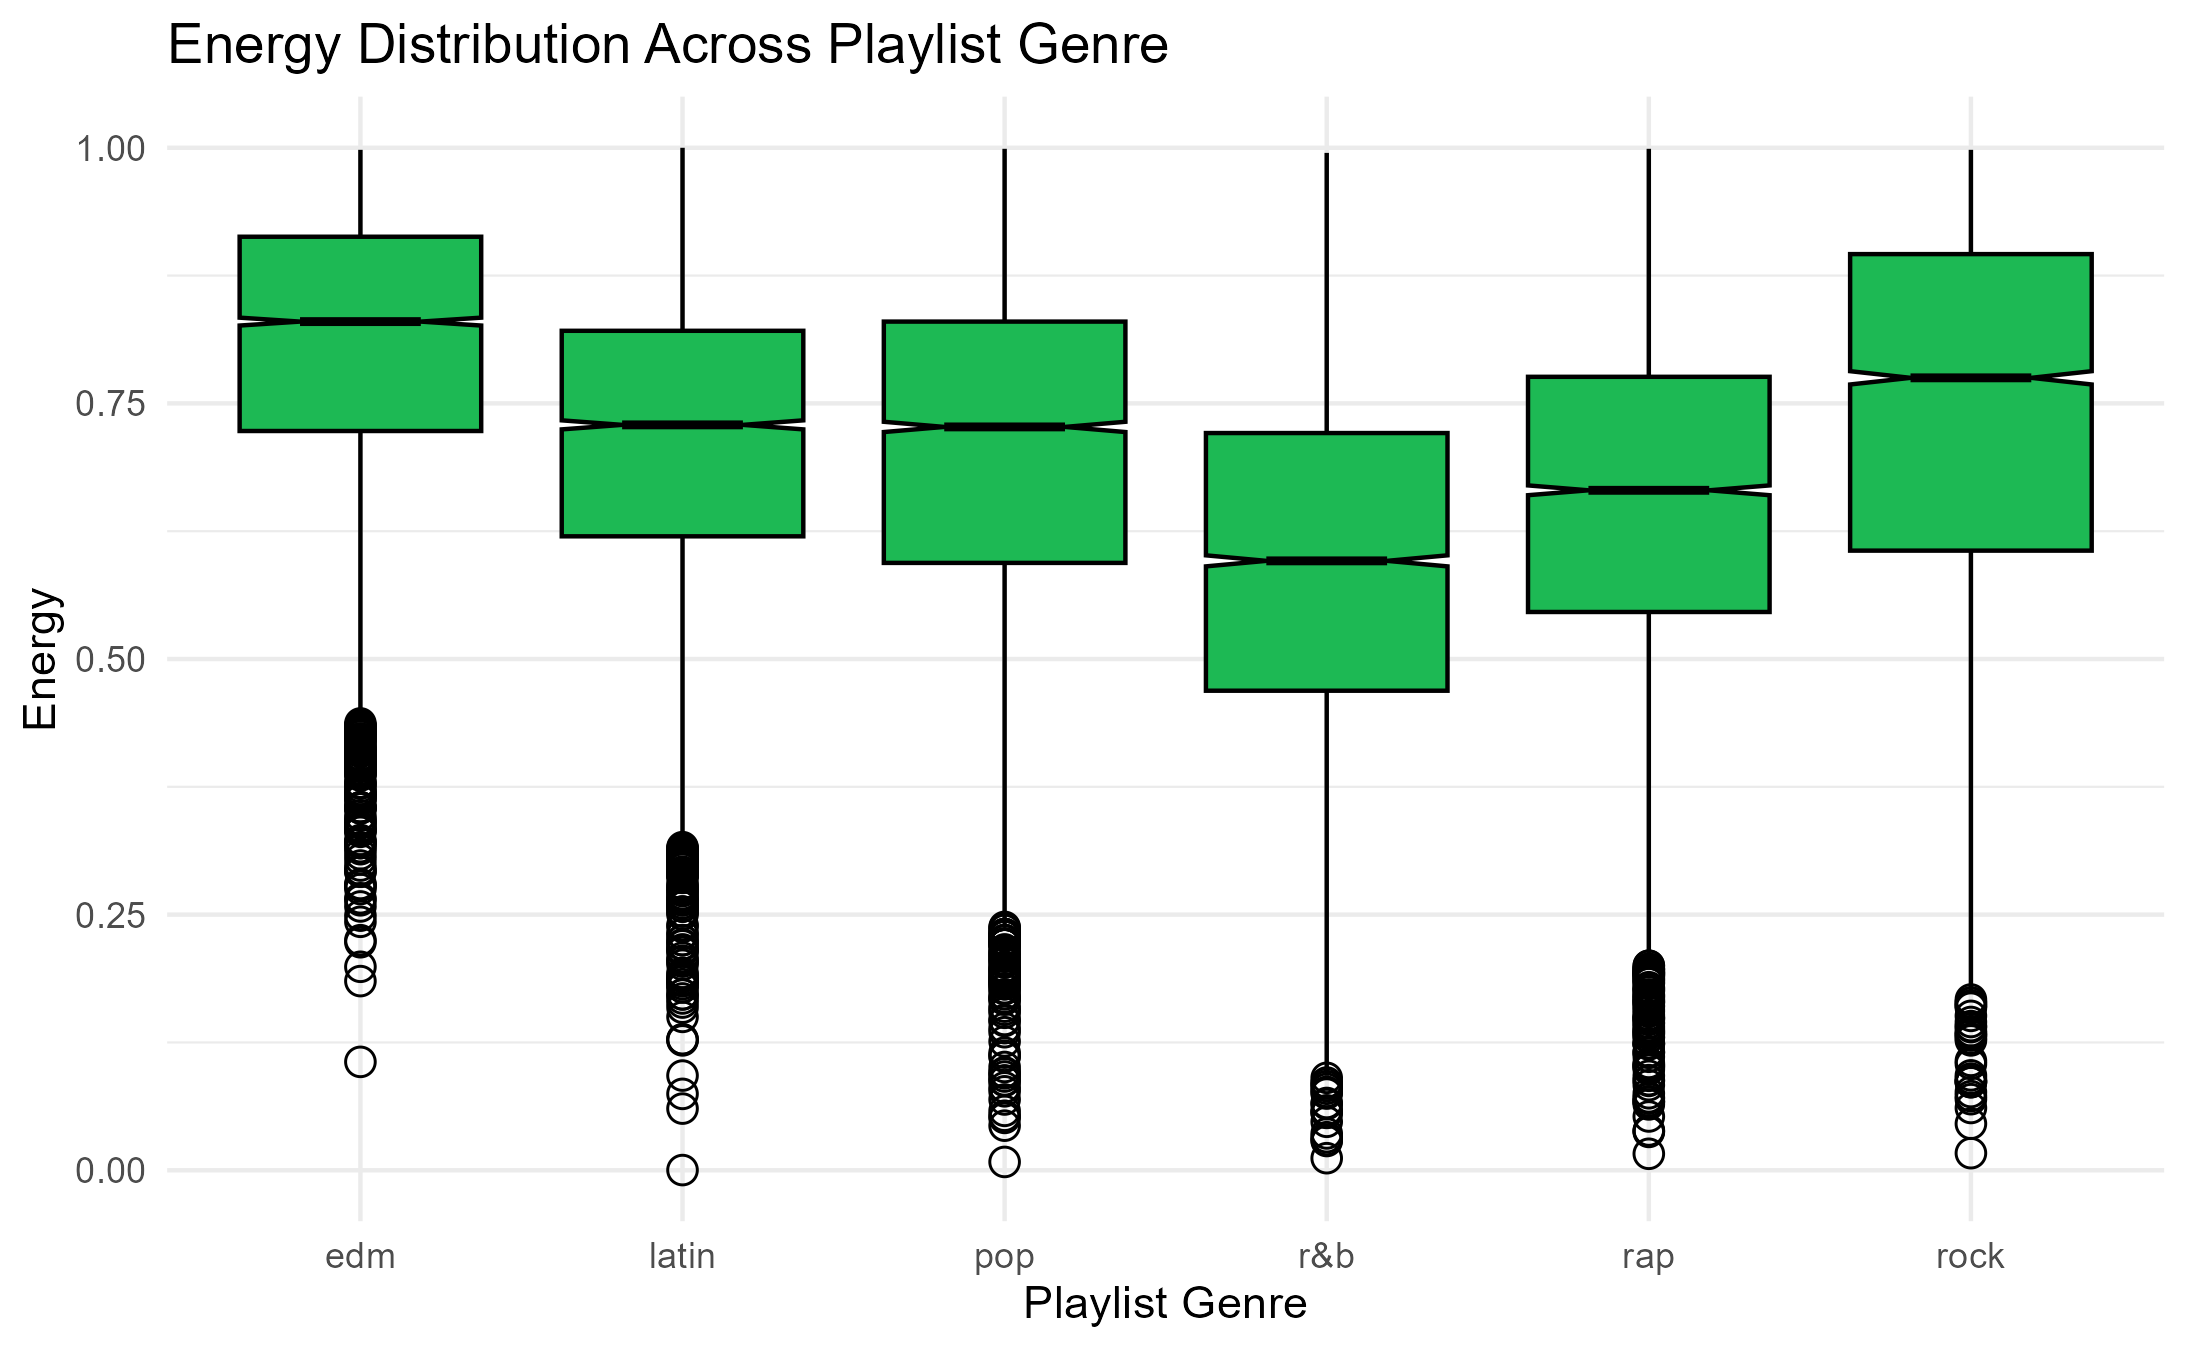
\includegraphics[scale=0.9]{slike/Genre-Energy.png}
		%veličina slike u odnosu na originalnu datoteku i pozicija slike
		\centering
		\caption{Distribucija energije kroz žanrove playlista}
		
	\end{figure}
	
	\subsubsection{5) Top 10 albuma prema popularnosti pjesama}
	
	\textbf{Opis grafa:}
	
	Na x osi nalazi se ime albuma, dok se na y osi nalazi prosječna popularnost pjesme u tom albumu. Vidimo kako su u prosjeku pjesme s albuma \textit{JACKBOYS, WHEN WE ALL FALL ASLEEP, WHERE DO WE GO?, The Academy, Rare} i ostali najpopularnije.
	
	
	\textbf{Slika grafa:}
	\begin{figure}[H]
		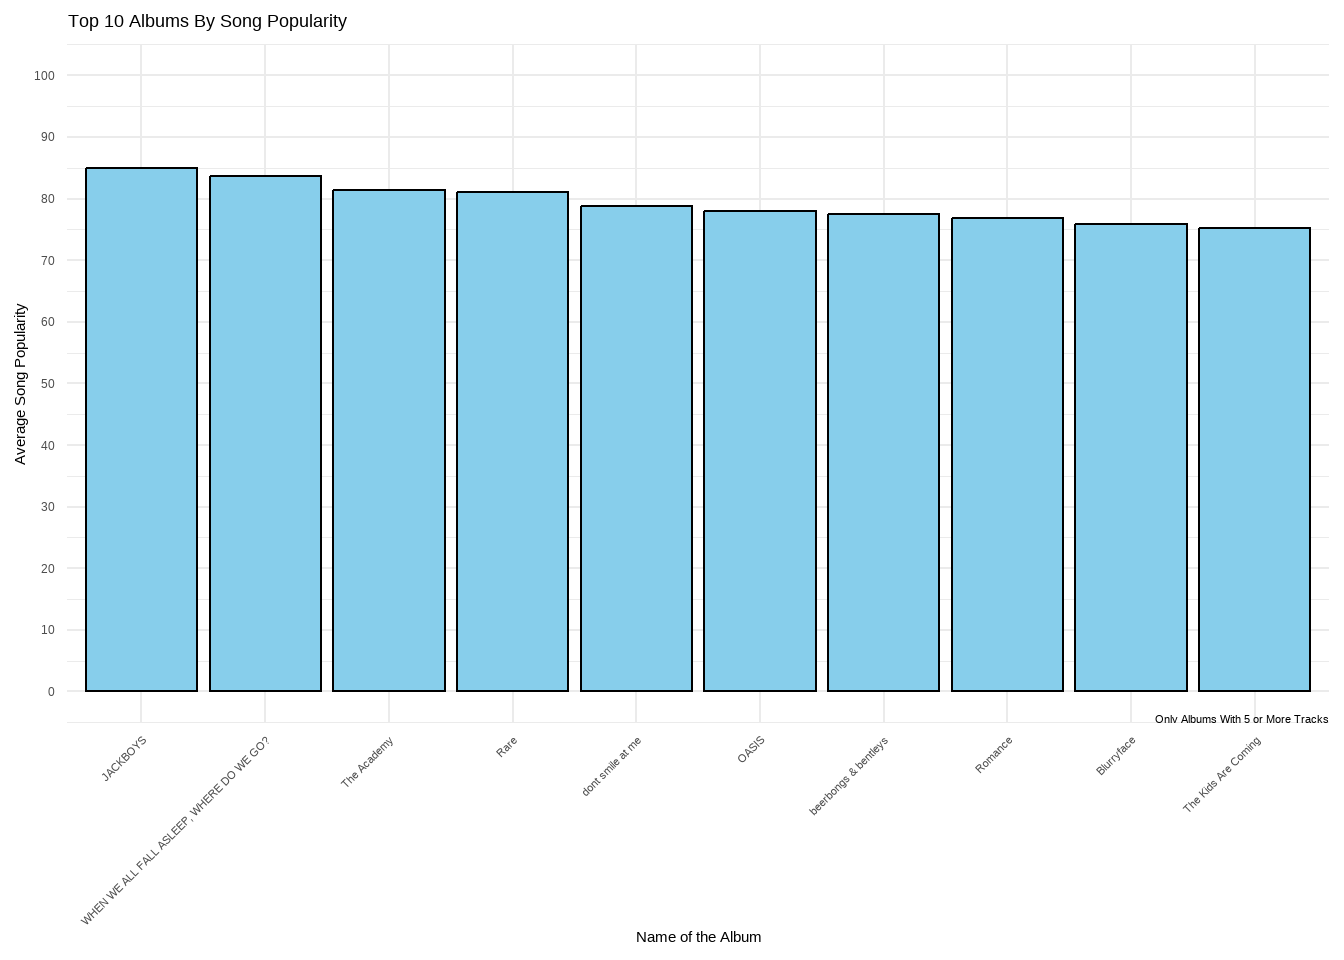
\includegraphics[scale=0.9]{slike/albums_by_song_popularity.png}
		%veličina slike u odnosu na originalnu datoteku i pozicija slike
		\centering
		\caption{Top 10 albuma prema popularnosti pjesama}
		
	\end{figure}
	
	\subsubsection{6) Top 10 playlista po popularnosti}
	
	\textbf{Opis grafa:}
	
	Na y osi nalaze se 10 najpopularnijih playlista, a na y os nam govori zbroj popularnosti svih pjesama u toj playlisti. Legenda prikazuje žanr pojedinih playlista. 
	Iz ovog grafa možemo zaključiti da dominiraju žanrovi: pop, R&B, rock i latin. Također, treba napomenuti da playlista s najvećom popularnošću pripada žanru Latin.
	
	\textbf{Slika grafa:}
	\begin{figure}[H]
		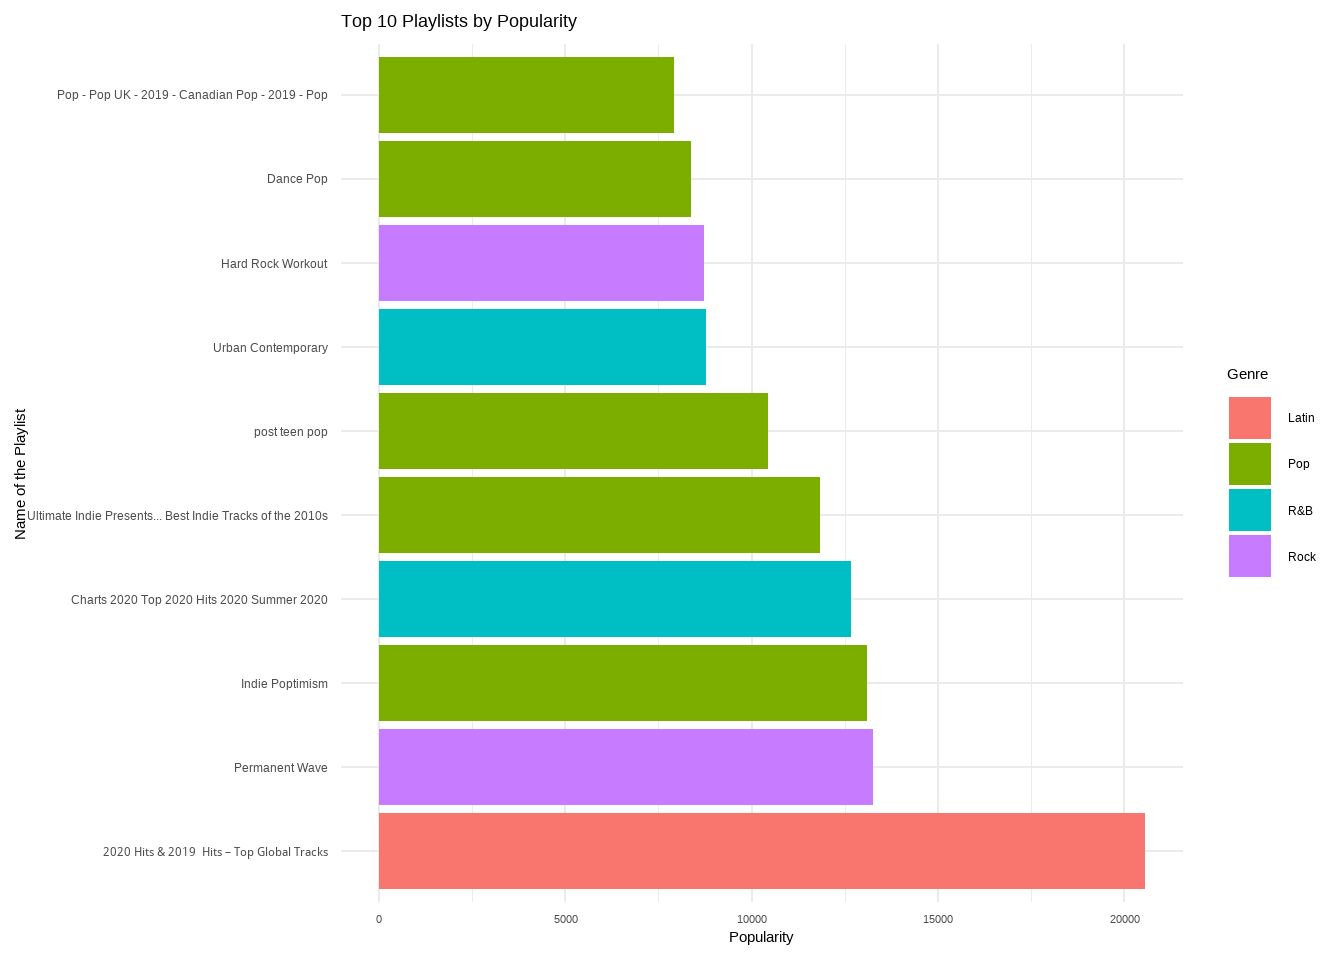
\includegraphics[scale=0.9]{slike/playlists_by_popularity.png}
		%veličina slike u odnosu na originalnu datoteku i pozicija slike
		\centering
		\caption{Top 10 playlista po popularnosti}
		
	\end{figure}
	
		\subsubsection{7) Distribucija žanrova i podžanrova}
	
	\textbf{Opis grafa:}
	
		Ovaj graf prikazuje broj playlista unutar određenih glavnih žanrova, razdijeljenih prema podžanrovima. Na x-osi su navedeni glavni žanrovi playlista, dok y-os pokazuje broj playlista. Svaki šareni segment na stupcu predstavlja određeni podžanr unutar glavnog žanra.
		
		Stupci su složeni jedan na drugi kako bi se vizualno prikazala distribucija podžanrova u okviru svakog glavnog žanra. 
	
	
	\textbf{Slika grafa:}
	\begin{figure}[H]
		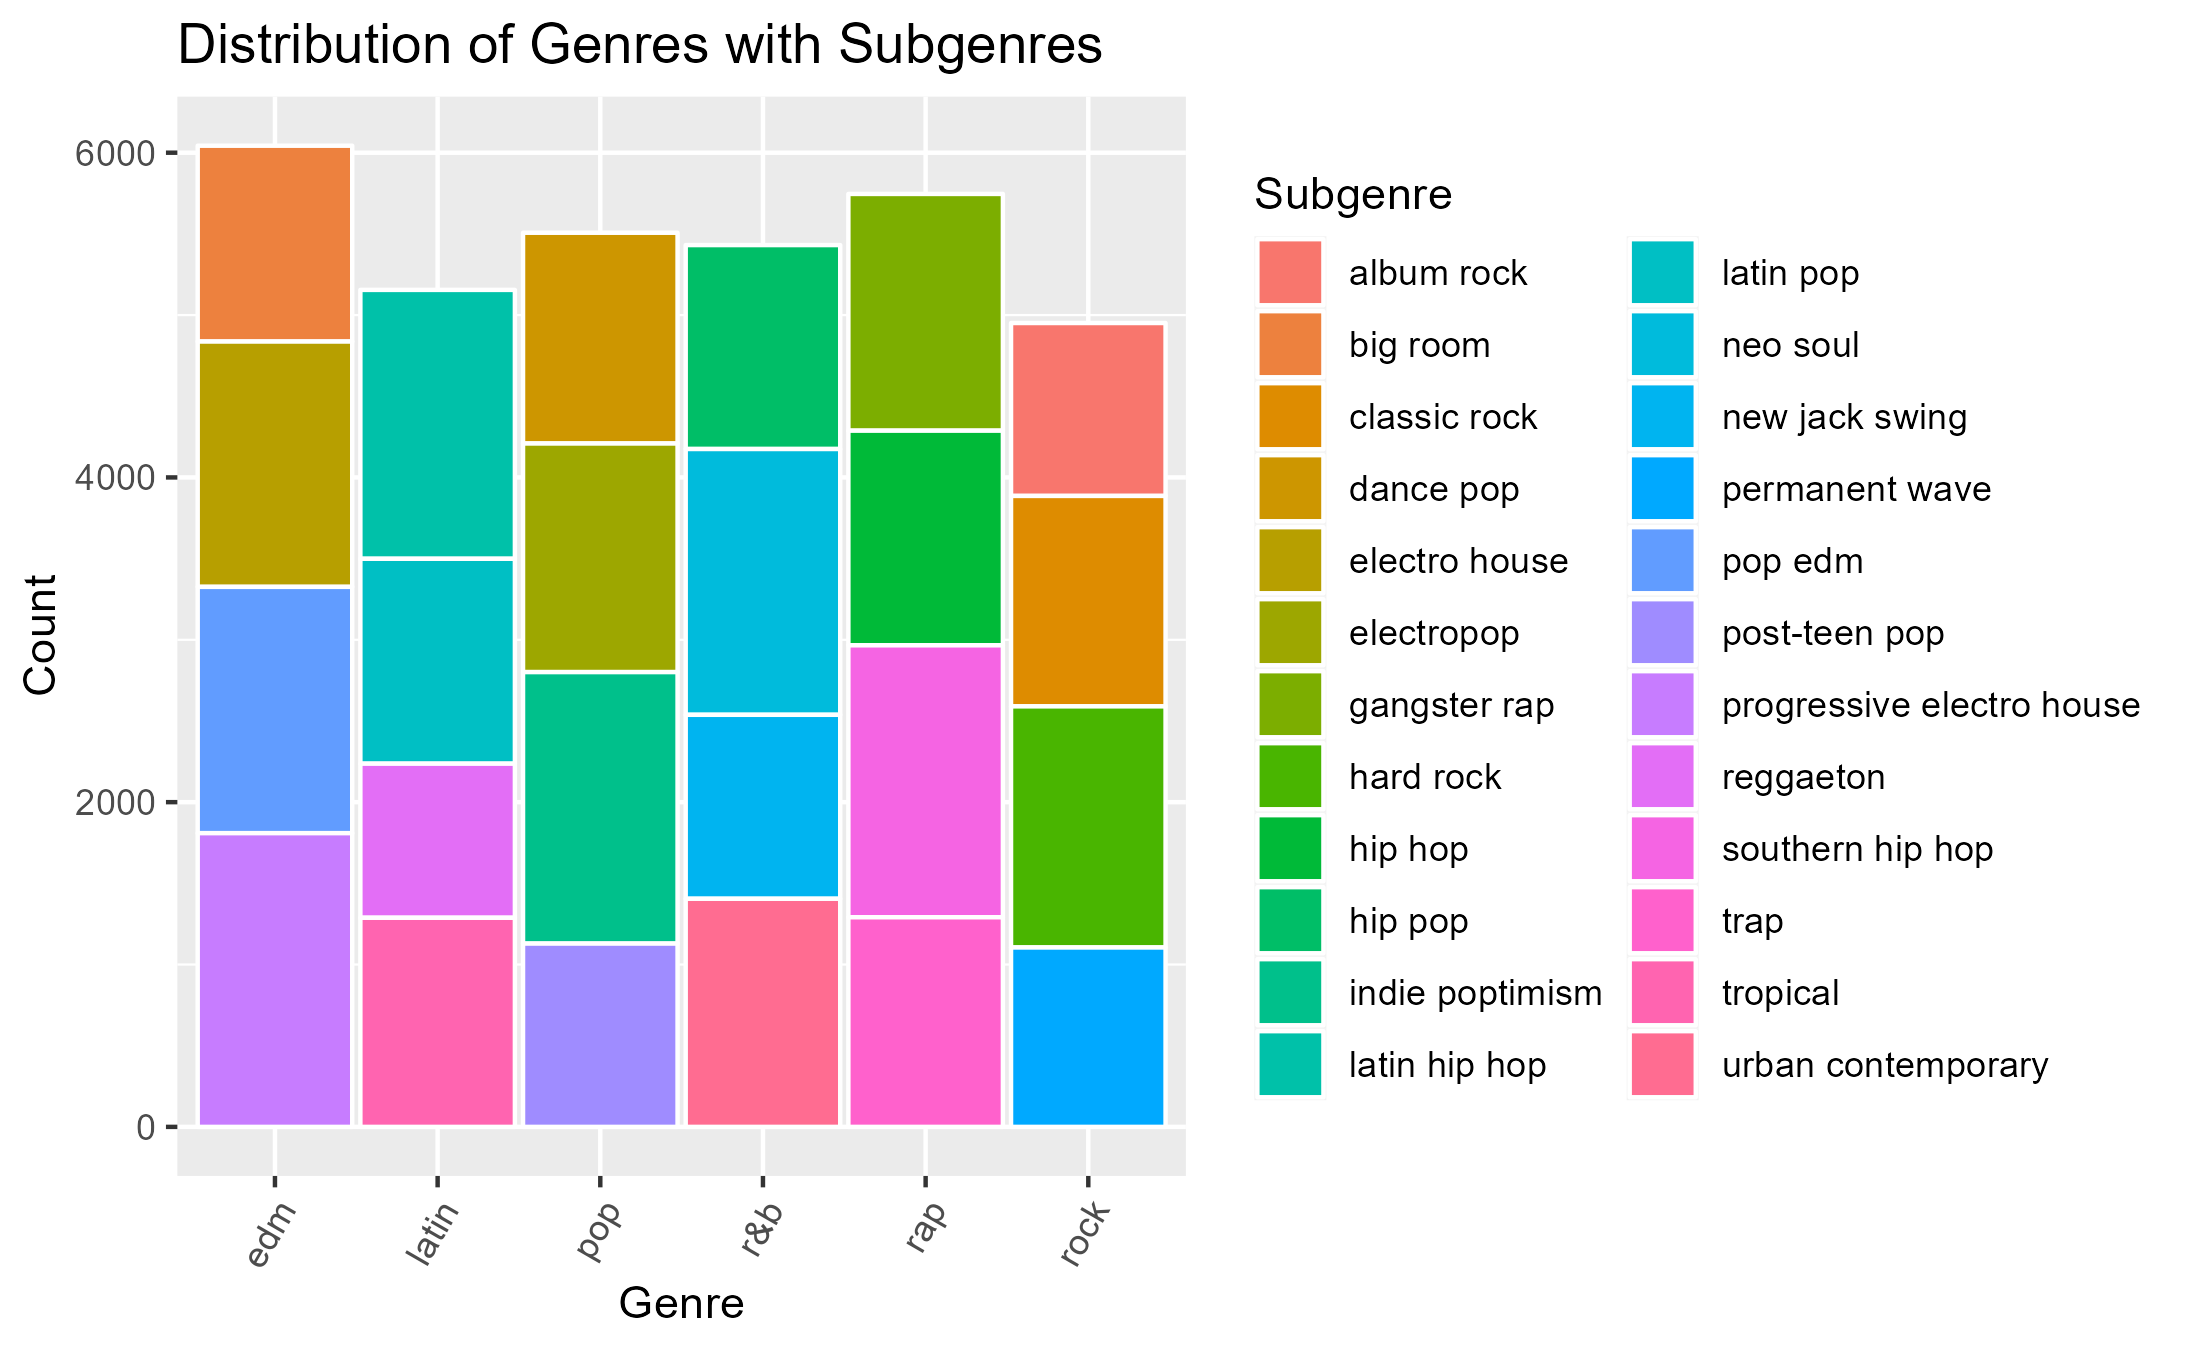
\includegraphics[scale=0.9]{slike/Genre-Subgenre.png}
		%veličina slike u odnosu na originalnu datoteku i pozicija slike
		\centering
		\caption{Distribucija žanrova i podžanrova}
		
	\end{figure}
	
	\subsubsection{8)  Prosječna popularnost pjesme po žanru}
	
	\textbf{Opis grafa:}
	
	Na grafu možemo vidjeti prosječnu popularnost pjesama grupiranih na osnovu žanra playliste u kojoj se nalaze. Možemo vidjeti kako su pop i latin najpopulaniji, dok je edm najmanje popularan među slušačima. 
	
	
	\textbf{Slika grafa:}
	\begin{figure}[H]
		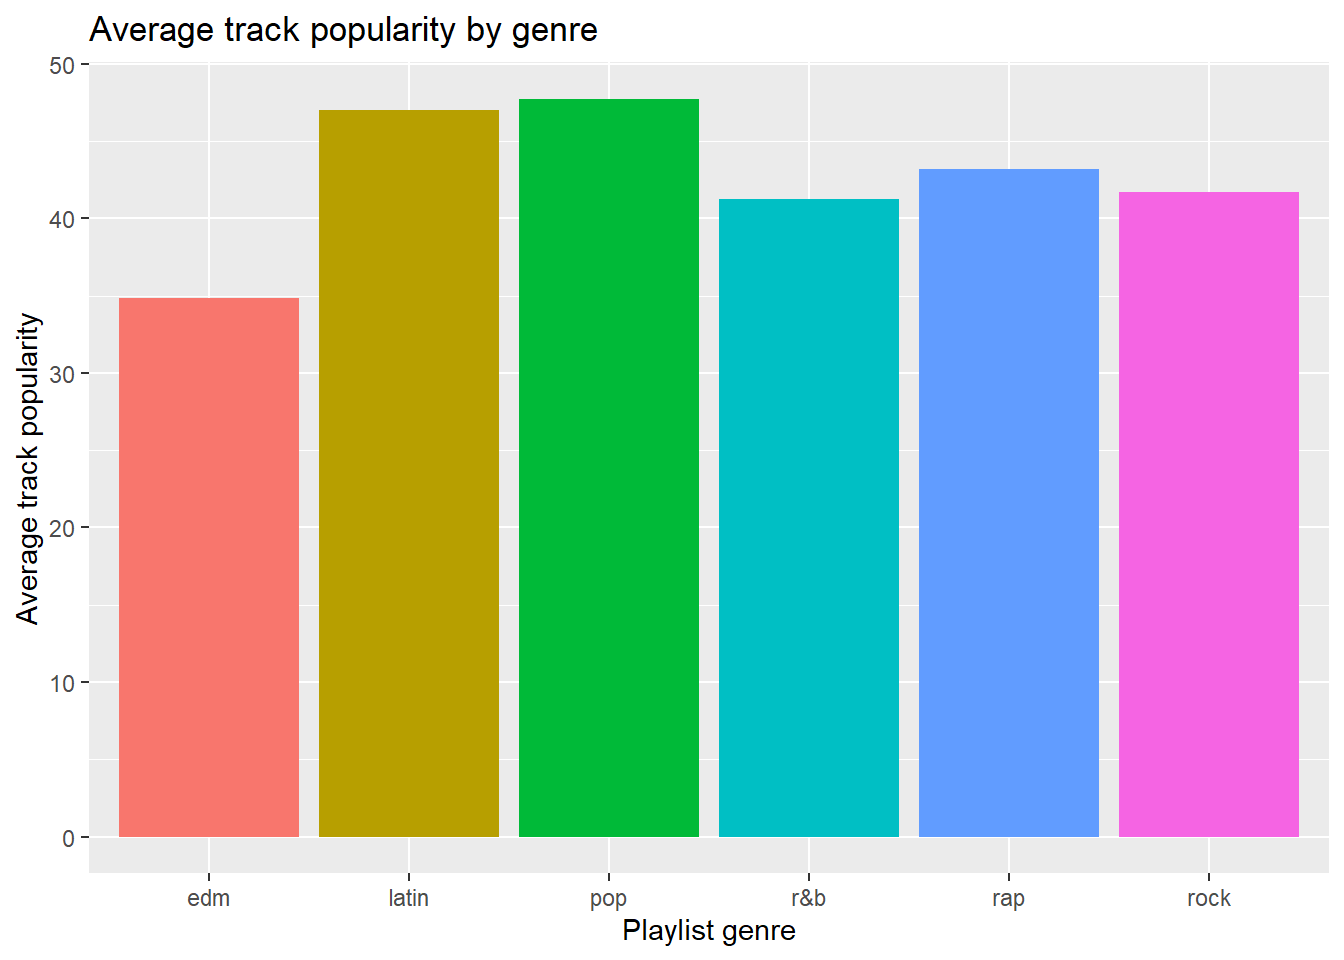
\includegraphics[scale=0.9]{slike/genre.png}
		%veličina slike u odnosu na originalnu datoteku i pozicija slike
		\centering
		\caption{ Prosječna popularnost pjesme po žanru}
		
	\end{figure}
	
	
	\subsubsection{9) Prosječna popularnost pjesme po podžanru}
	
	\textbf{Opis grafa:}
	
	Na ovome grafu možemo vidjeti prikaz sličan kao i na prethodnom, međutim sada su pjesme grupirane na temelju podžanra. Boje stupaca označavaju vrstu žanra, kako bismo bolje vidjeli popularnost pojedinih podžanrova s obzirom na njihov žanr.
	Vidimo kako se ističe post-teen pop, iz čega bi mogli zaključiti da su velik broj korisnika Spotifyja mladu ljudi nakon tinejdžerske dobi.
	
	\textbf{Slika grafa:}
	\begin{figure}[H]
		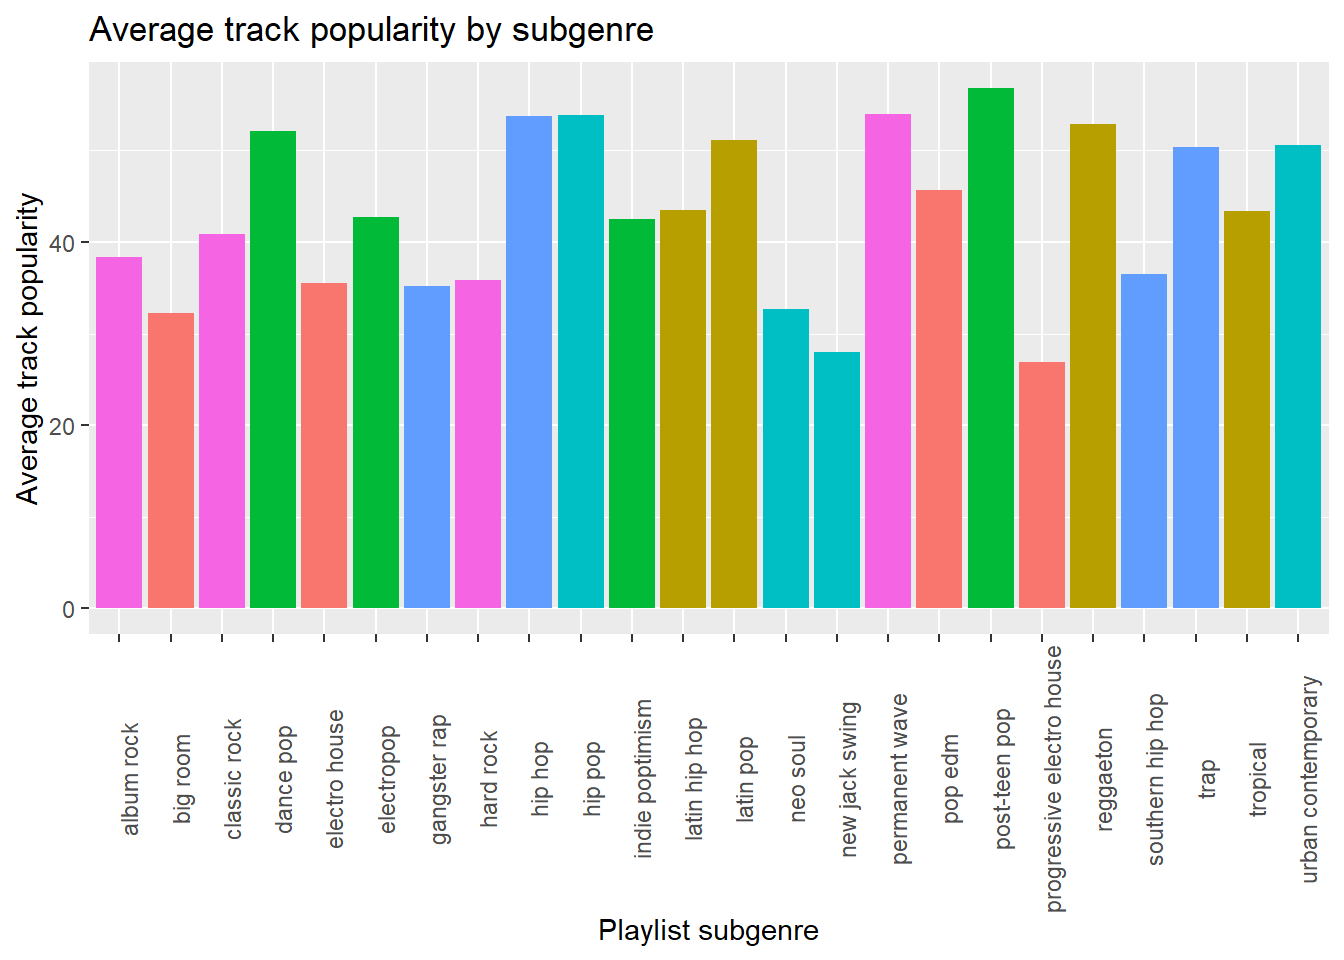
\includegraphics[scale=0.9]{slike/subgenre.png}
		%veličina slike u odnosu na originalnu datoteku i pozicija slike
		\centering
		\caption{Prosječna popularnost pjesme po podžanru}
		
	\end{figure}


		\subsubsection{10) Odnos između energije i valencije u odnosu na žanr}
    
    \textbf{Opis grafa:}
    
    	Ovaj graf prikazuje odnos između energije i valencije. N a x-osi nalazi se energija koja može biti u rasponu između 0 i 1, a na y-osi nalazi se valencija koja može biti u isto rasponu kao i energija. Svaka točka na grafu prikazuje jednu pjesmu , a njezina pozicija prikazuje odnos energija-valencija. Svaka boja točke prikazuje različiti žanr. 
    	Iz grafa je vidljivo da je valencija ravnomjerno raspoređena među različitim žanrovima, dok se energija koncentrira s obzirom na specifične žanrove.
    
    \textbf{Slika grafa:}
    \begin{figure}[H]
        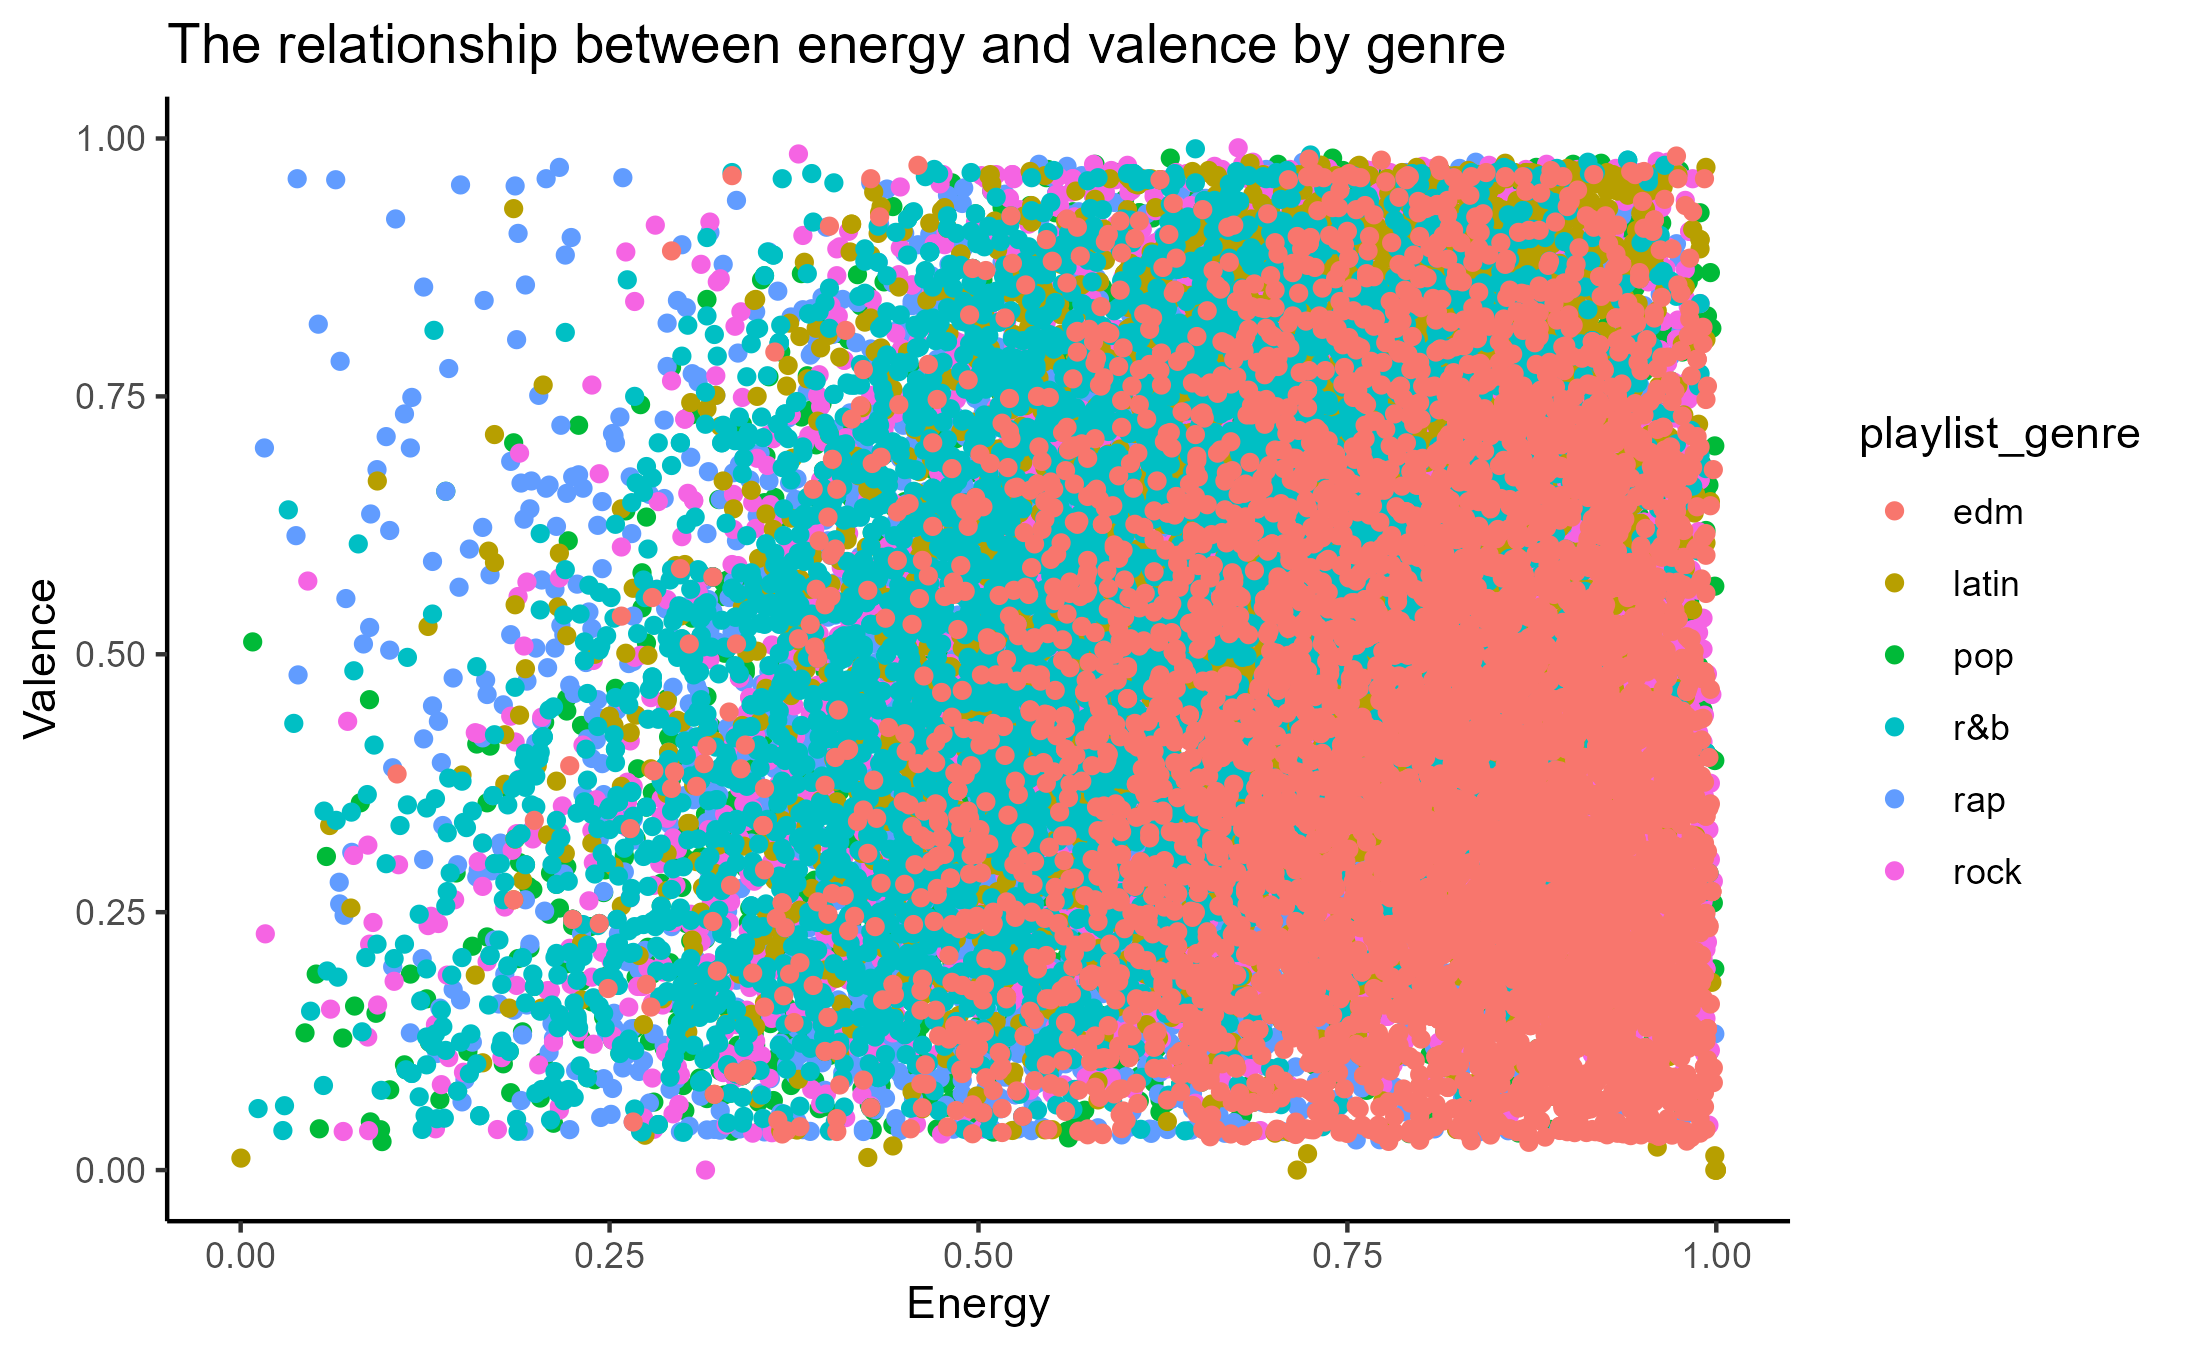
\includegraphics[scale=0.9]{slike/The relationship between energy and valence by genre.png}
        %veličina slike u odnosu na originalnu datoteku i pozicija slike
        \centering
        \caption{Odnos između energije i valencije u odnosu na žanr}
        
    \end{figure}

	
		\subsubsection{11) Odnos energije i plesnosti za različite popularnosti pjesama}
	
	\textbf{Opis grafa:}
	
	Ovaj šareni graf prikazuje odnos između plesnosti (x-os) i energije (y-os) za različite glazbene pjesme. Svaka točka na grafu predstavlja pojedinu pjesmu, a njezina boja označava razinu popularnosti. Tamnije crvene nijanse označavaju popularnije pjesme, dok svjetlije plave nijanse ukazuju na manju popularnost.
	
	Graf pruža uvid u raznolikost glazbenih preferencija te naglašava da glazbene osobitosti kao što su plesnost i energija nisu nužno ključni faktori koji određuju popularnost pjesama na temelju analize ovog skupa podataka.
	
	\textbf{Slika grafa:}
	\begin{figure}[H]
		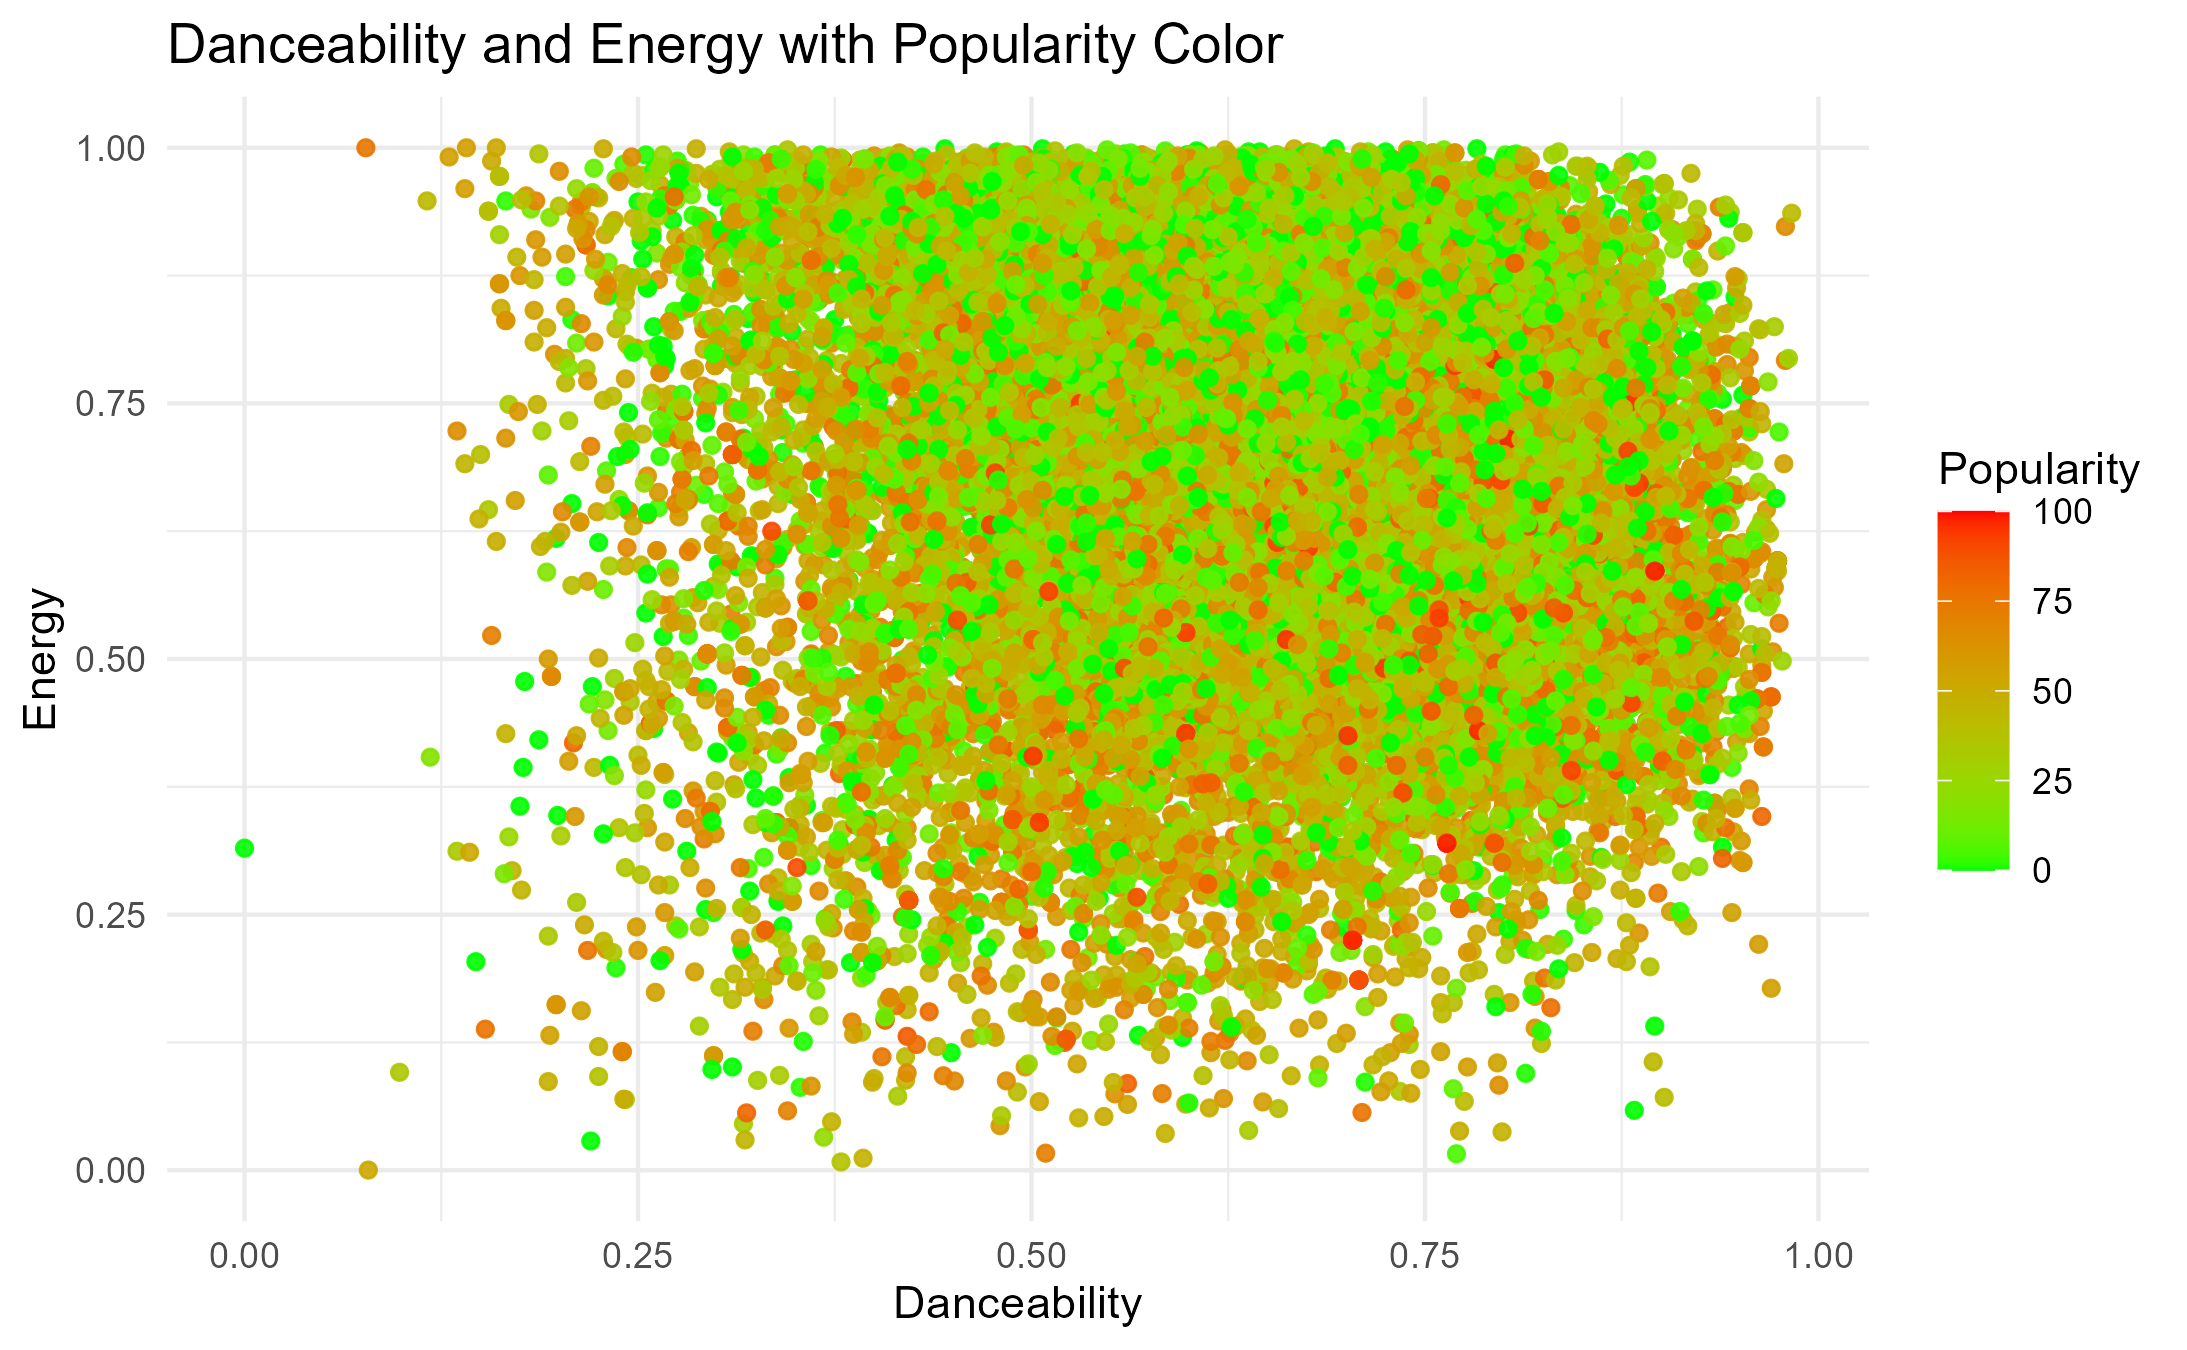
\includegraphics[scale=0.9]{slike/Dance-Energy-popularity.png}
		%veličina slike u odnosu na originalnu datoteku i pozicija slike
		\centering
		\caption{ Odnos energije i plesnosti za različite popularnosti pjesama}
		
	\end{figure}


	\subsubsection{12) Histogram trajanja pjesama}
    
    \textbf{Opis grafa:}
    
Ovaj graf pruža uvid u distribuciju trajanja pjesama. Na x-osi nalaze se različite razine trajanju u sekundama, dok y-os predstavlja broj pjesma u pojedinoj razini. Ovaj zanimljiv histogram omogućava vizualnu interpretaciju o najčešćem trajanju pjesama.
Iz grafa možemo zaključiti da većina pjesama ima trajanje od otprilike 3.5 minute.
    

    \textbf{Slika grafa:}
    \begin{figure}[H]
        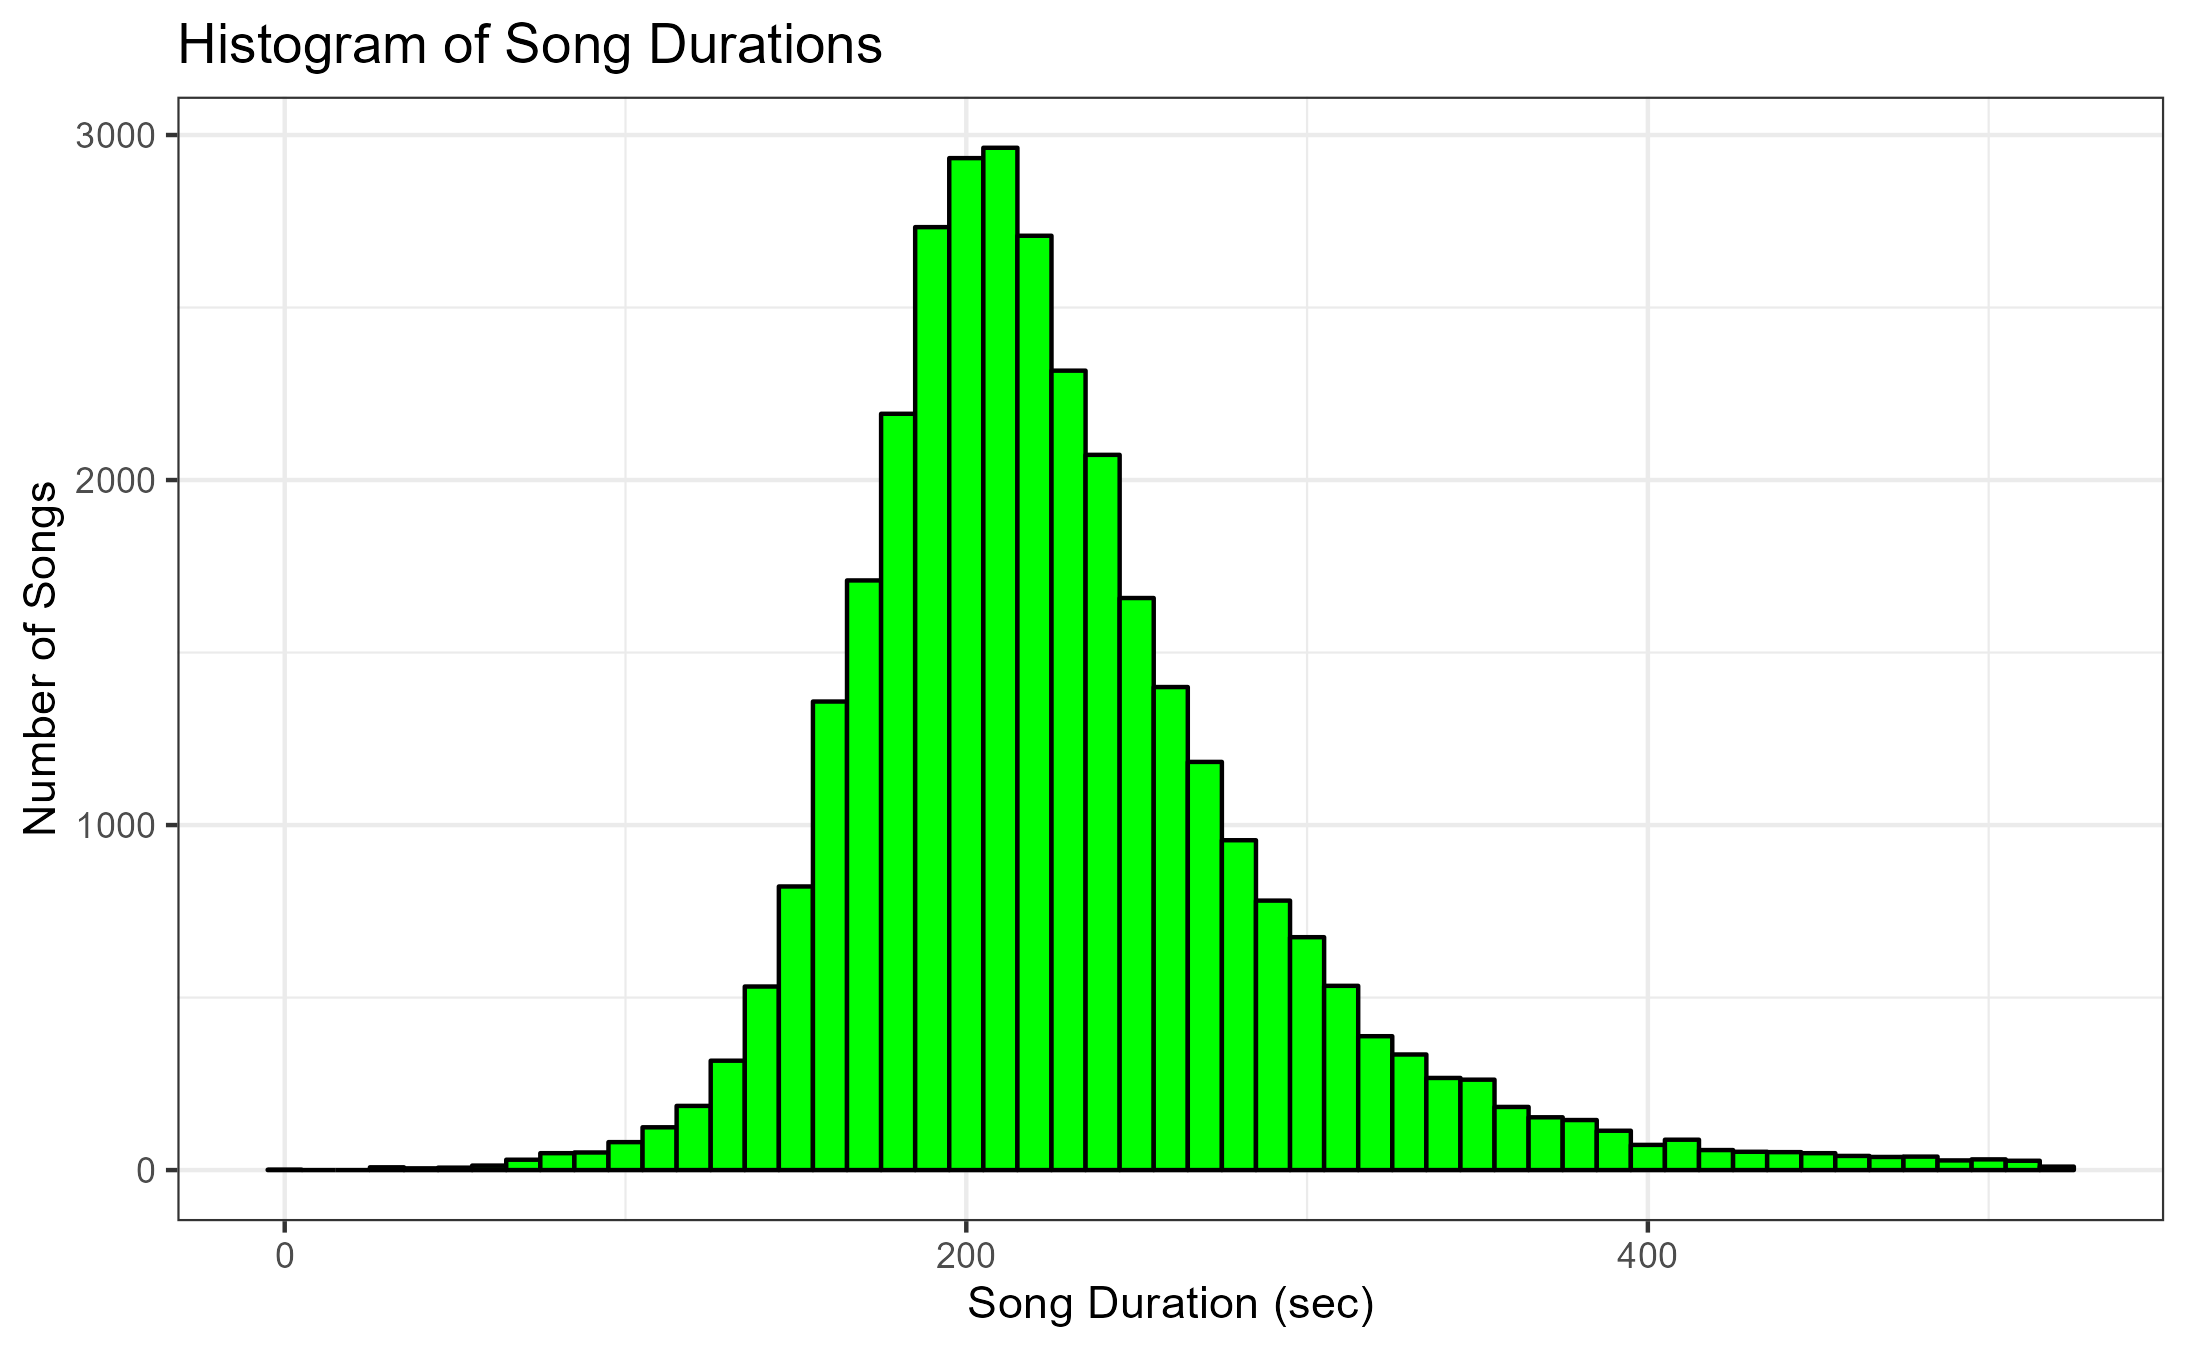
\includegraphics[scale=0.9]{slike/Histogram of song durations.png}
        %veličina slike u odnosu na originalnu datoteku i pozicija slike
        \centering
        \caption{Histogram trajanja pjesama}
        
    \end{figure}
    
    \subsubsection{13) Odnos energije pjesme i njene popularnosti}
    
    \textbf{Opis grafa:}
    
    Graf prikazuje odnos pupularnosti pjesme s njenom energijom. Vidimo kako se linija energije uglavnom kreće oko vrijednosti 0.7, dok je vidljiv mali pad do vrijednosti 0.6 prema kraju x-osi, te ponovno porast do vrijednosti 0.7 na kraju grafa. Ove veće oscilacije na kraju grafa možemo pripisati manjem broju pjesama s velikom vrijednosti varijable \textit{popularity}.
    
    
    \textbf{Slika grafa:}
    \begin{figure}[H]
    	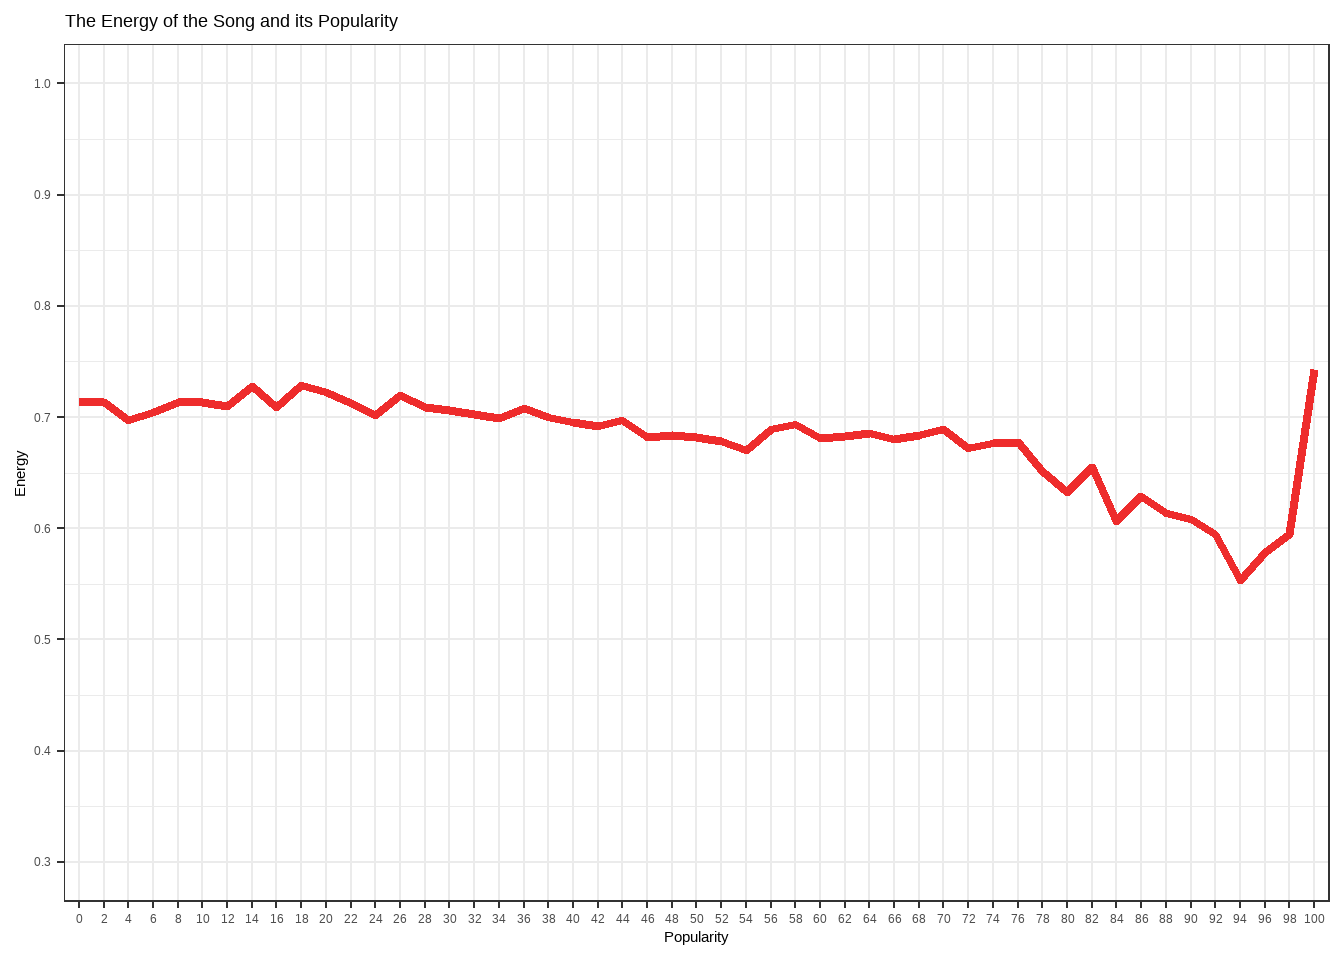
\includegraphics[scale=0.9]{slike/energy_popularity.png}
    	\centering
    	\caption{Odnos energije pjesme i njene popularnosti}
    	
    \end{figure}
    
    \subsubsection{14) Odnos energije pjesme i njezine plesnosti}
    
    \textbf{Opis grafa:}
    
    Graf prikazuje odnos popularnosti pjesme s njenom plesnošću. Ovdje je funkcija koja prikazuje plesnost uglavnom ravnomjerno raspoređena oko vrijednosti 0.65, dok je s porastom popularnosti vidljiv blagi porast funkcije.
    
    
    \textbf{Slika grafa:}
    \begin{figure}[H]
    	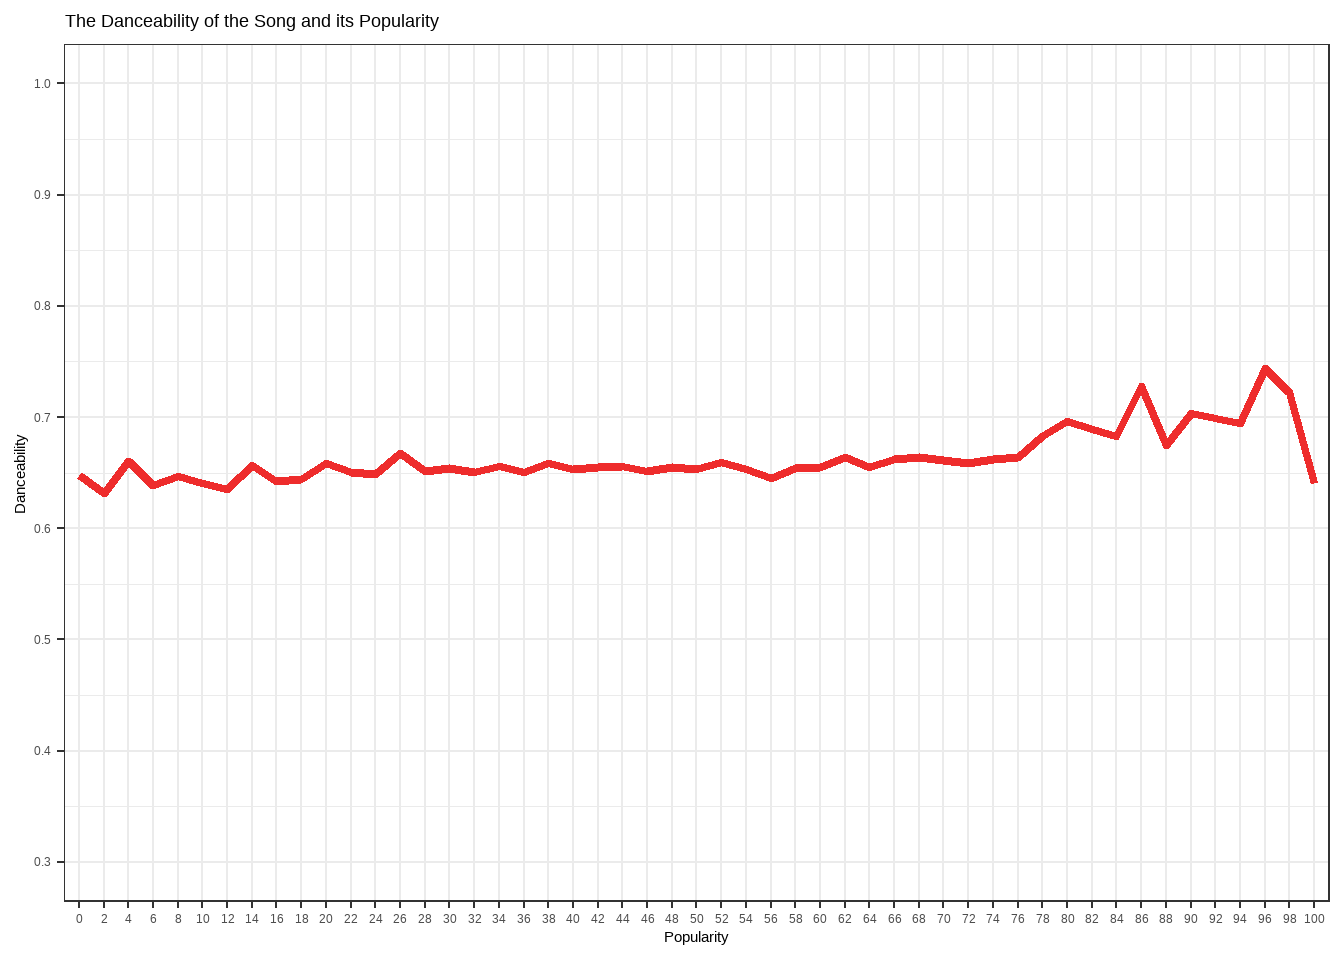
\includegraphics[scale=0.9]{slike/danceability_popularity.png}
    	\centering
    	\caption{Odnos energije pjesme i njezine plesnosti}
    	
    \end{figure}
    
    

\clearpage
\section{Prediktivni modeli}

	U nastavku bit će opisan rad s osnovnim prediktivnim modelima: linearna regresija te kNN klasifikacija. 
	
	\subsection{Linearna regresija}
	
	Linearna regresija koristi se za predviđanje vrijednosti varijable s obzirom na vrijednosti jedne ili više drugih. Za određivanje koeficijenata smjera koristi se metoda najmanjih kvadrata. U nastavku ćemo pokušati predvidjeti vrijednost varijable \textit{energy} s pomoću ostalih numeričkih varijabli iz našeg podatkovnog skupa, tj.koristit ćemo višestruku (multiplu) linearnu regresiju.
	Za početak provjerit ćemo vrijednosti kolinearnosti ulaznih varijabli.
	
	\begin{figure}[H]
		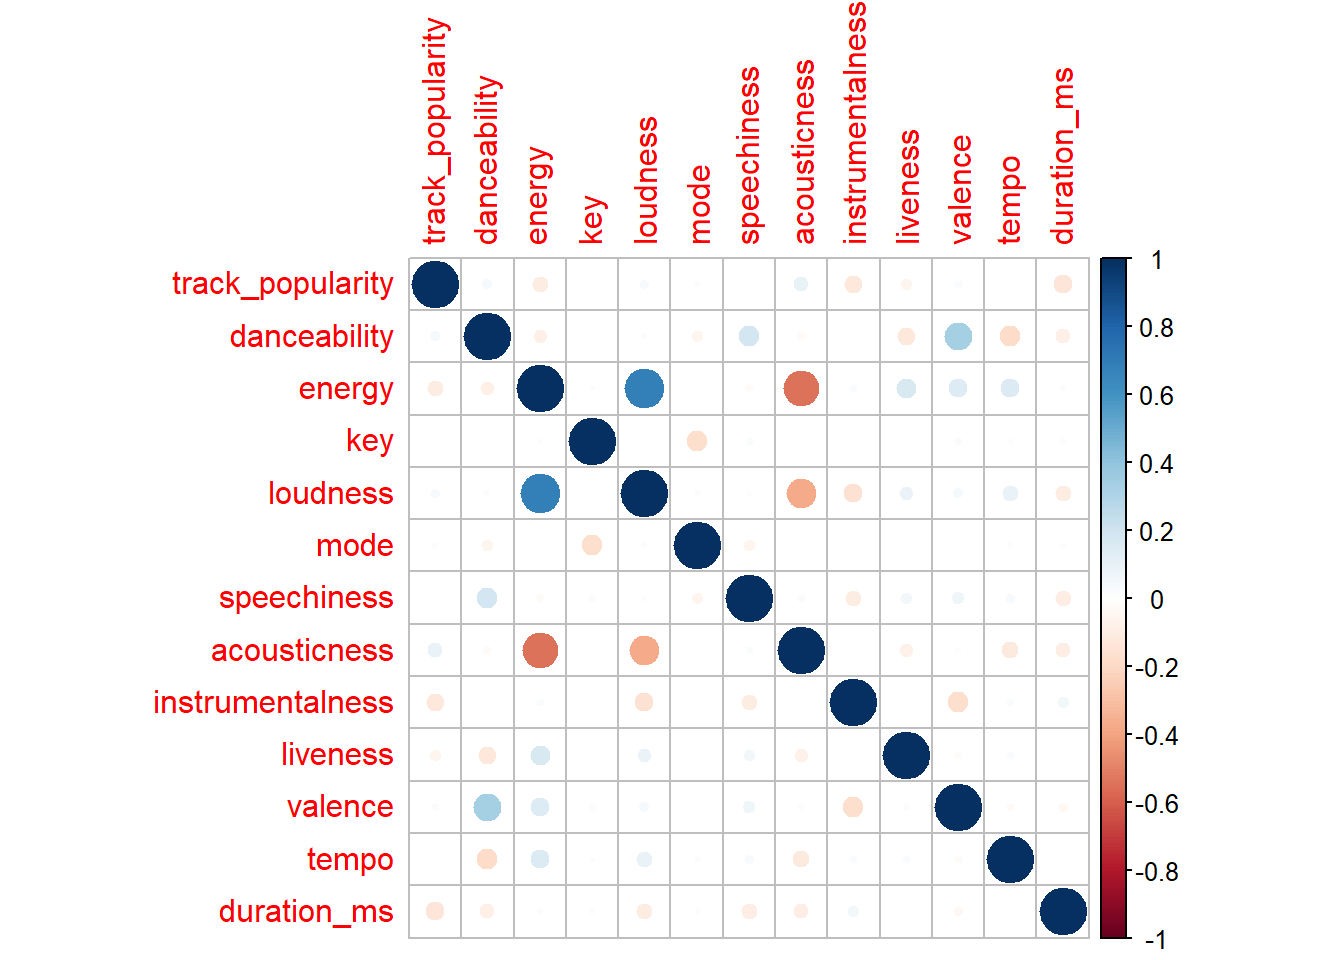
\includegraphics[scale=0.9]{slike/corrplot.png}
		%veličina slike u odnosu na originalnu datoteku i pozicija slike
		\centering
		\caption{Korelacije ulaznih varijabli}
		
	\end{figure}
	
	Možemo primijetiti da nema prevelikih kolinearnosti, a vidimo da npr. \textit{valence} i \textit{danceability} imaju  pozitivnu korelaciju, što nam govori da je moguće da "plesne" pjesme imaju veću valenciju, tj. pozitivnost.
	S druge strane, \textit{acousticness} i \textit{loudness} imaju negativnu korelaciju, što znači da akustične trake većinom imaju manju glasnoću.
	
	Za provjeru moguće multikolinearnosti koristit ćemo VIF mjeru koju ćemo izračunati i čiji rezultat se nalazi u nastavku:
	
	\begin{figure}[H]
		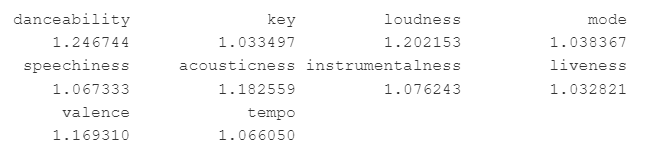
\includegraphics[scale=0.9]{slike/vif.png}
		%veličina slike u odnosu na originalnu datoteku i pozicija slike
		\centering
		\caption{VIF}
		
	\end{figure}
	
	Na temelju izračunatih vrijednosti možemo zaključiti da vrlo vjerojatno nema multikolinearnosti ulaznih varijabli
	
	Sada ćemo konačno stvoriti linearni model. Kao što je već navedeno, varijabla \textit{energy} bit će izlaz, a preostale numeričke varijable ulazi u modelu.
	Podatkovni okvir razdijeljen je u 2 dijela, jedan za treniranje te jedan za testiranje modela. Veličina okvira za treniranje je 70\% originalnog podatkovnog okvira. 
	U nastavku prvo slijedi sažetak korištenog linearnog modela.
	
	\begin{figure}[H]
		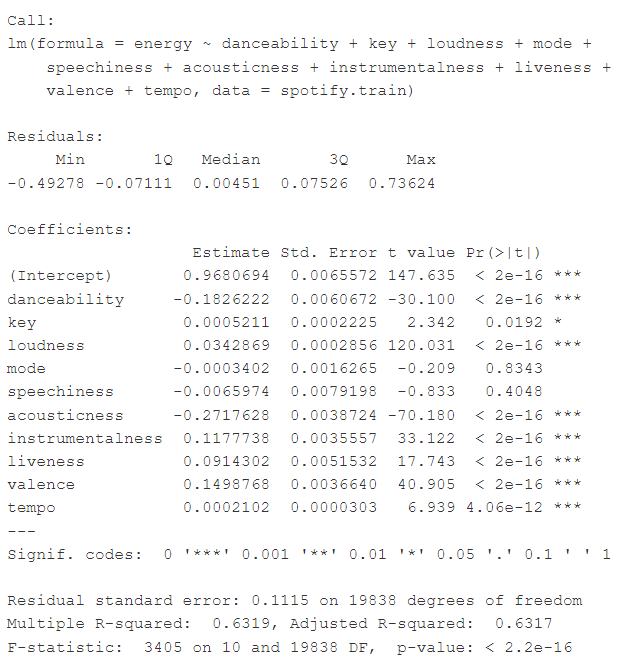
\includegraphics[scale=0.9]{slike/linReg.png}
		%veličina slike u odnosu na originalnu datoteku i pozicija slike
		\centering
		\caption{Sažetak linearnog modela}
		
	\end{figure}
	
	Možemo vidjeti da su \textit{danceability, loudness, acousticness, instrumentalness, livenes} i \textit{valence} jako statistički značajni u ovome modelu, \textit{key} ima manje statistički značajan utjecaj, dok \textit{mode} i \textit{speechiness} vrlo vjerojatno nemaju statističkog utjecaja na ovaj model, zbog visoke p-vrijednosti.
	
	Rezidualna standardna pogreška (RSE) nam govori koliko u prosjeku model promašuje kod predviđanja izlazne varijable \textit{energy}, a vidimo da iznosi 0.1115.
	
	\textit{Multiple R-squared} i \textit{Adjusted R-squared} iznose 0.6319, odnosno 0.6317. R-kvadrat nam govori o količini varijabilnosti koja je objašnjena modelom, a u našem modelu možemo zaključiti da je otprilike 63\% varijabilnosti varijable \textit{energy} objašnjeno modelom. Kako smo koristili višestruku linearnu regresiju više pažnje obratit ćemo na prilagođenu R-kvadrat vrijednost koja prilagođava R-kvadrat mjeru zbog broja prediktora u modelu, međutim vidimo da su otprilike iste.
	
	Konačno, F-statistika s p-vrijednosti manjom od \(2.2 \times 10^{-16}\) nam govori da je model statistički značajan u objašnjavanju izlazne varijable.
	
	
	Sada ćemo koristeći model koji je istreniran nad trening skupom pokušati procijeniti vrijednosti varijable \textit{energy} u testnom podatkovnom okviru. Kako bismo provjerili kvalitetu našeg modela, iskoristit ćemo RMSE (\textit{engl. root mean square error}) mjeru koja iznosi 0.1138, što je otprilike isto kao kod rezidualne pogreške.
	
	U nastavku ćemo iskoristit metodu \textit{augment} iz paketa \textit{broom} koja na osnovu prosljeđenog prediktivnog modela vraća originalni podatkovni okvir korišten za stvaranje modela, ali proširen sa nizom korisnih stupaca:
	\begin{itemize}
		\item \texttt{.fitted} - Predikcije dobivene primjenom modela
		\item \texttt{.se.fit} - Standardna greška pojedine predikcije
		\item \texttt{.resid} - Iznos reziduala
		\item \texttt{.std.resid} - Reziduali standardizirani na interval [0,1]
		\item \texttt{.hat} - Mjera “ekstremnosti” ulazne varijable obzervacije
		\item \texttt{.cooksd} - Mjera “utjecajnosti” obzervacije na model
	\end{itemize}
	
	U nastavku prikazano je nekoliko grafova koji su redom: točkasti graf sa predikcijama na osi x i (standardiziranim) rezidualima na osi y, graf funkcije gustoće razdiobe standardiziranih reziduala, kvantil-kvantil graf standardiziranih reziduala
	reziduala.
	
	\begin{figure}[H]
		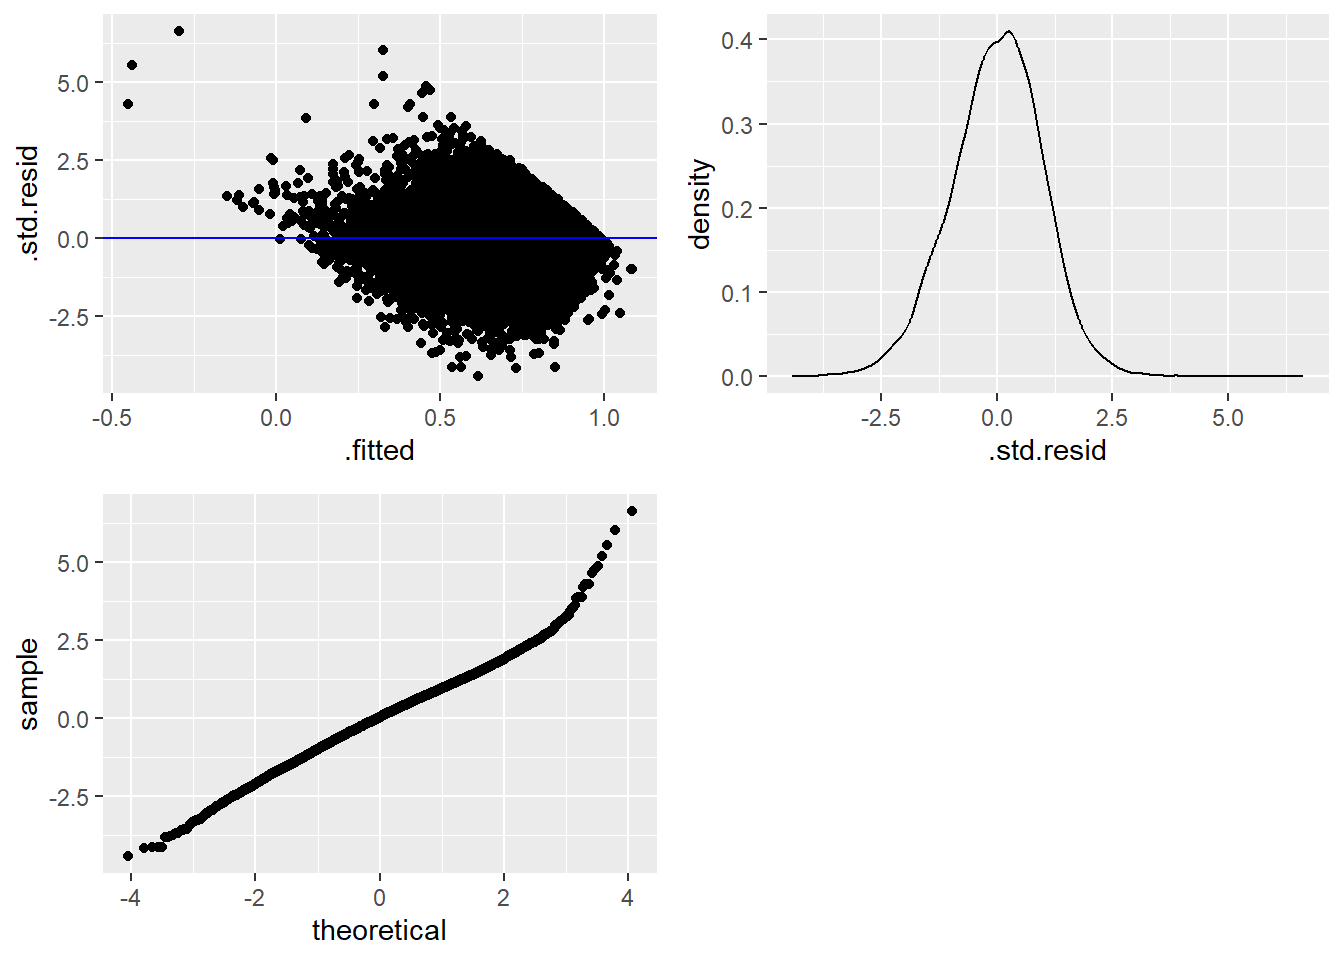
\includegraphics[scale=0.9]{slike/predikcije.png}
		%veličina slike u odnosu na originalnu datoteku i pozicija slike
		\centering
		\caption{Vizualizacije linearnog modela}
		
	\end{figure}
	
	Na temelju ovih vizualizacija te već prethodno navedenih svojstava linearnog modela možemo zaključiti da je linearni model koji smo dobili vrlo vjerojatno dobar dobar izbor za stvaranje predikcija. 
	
	\subsection{kNN klasifikacija}
	
	Ovaj klasifikacijski prediktivni model koristit ćemo za predviđanje kategorijske varijable \textit{genre}. Kako se određena pjesma može nalaziti na više playlista, a svaka playlista može imati drugačiji žanr, za početak ćemo odrediti da ako se pjesma nalazi na više playlista, sve te retke ćemo spojiti u jedan koji će pjesmi pridružiti onaj žanr na kojem pjesma ima najviše playlista. 
	
	Kao i kod linearne regresije podatkovni okvir bit će razdijeljen u trening i test ovkir. Također, kako je ovo klasifikacijski model podrazumijeva se da je ciljna varijabla \textit{genre} faktorizirana varijabla. Također sve numeričke varijable bit će normalizirane i svedene na istu skalu vrijednosti. 
	
	Kako je već navedeno, izlazna varijabla bit će \textit{genre}, a ulazne sve numeričke varijable u okviru, tj. \textit{track\_popularity, danceability, energy, key, loudness, mode, speechiness, acousticness, instrumentalness, liveness, valence, tempo, duration\_ms}
	
	Kako bismo provjerili uspješnost modela koristit ćemo matricu konfuzije čiji izgled se nalazi u nastavku. Retci označavaju stvarne vrijednosti, a stupci predviđene vrijednosti.
	
	\begin{figure}[H]
		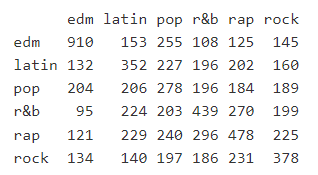
\includegraphics[scale=0.9]{slike/confMatrix.png}
		%veličina slike u odnosu na originalnu datoteku i pozicija slike
		\centering
		\caption{Confusion matrix}
		
	\end{figure}
	
	Sada ćemo prikazati ovu matricu kao \textit{heatmap}
	
	\begin{figure}[H]
		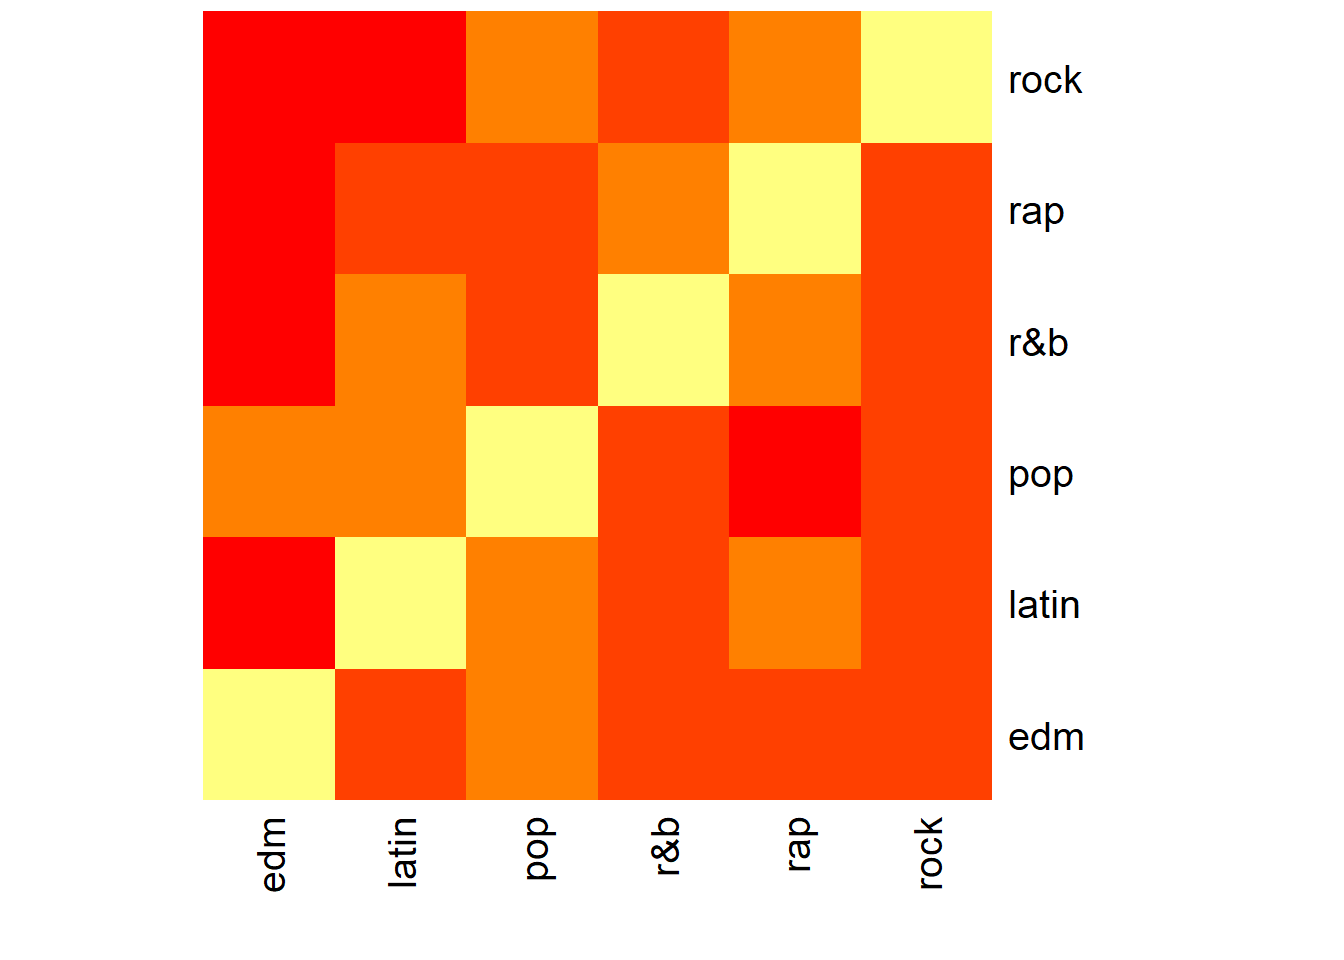
\includegraphics[scale=0.9]{slike/heatmap.png}
		%veličina slike u odnosu na originalnu datoteku i pozicija slike
		\centering
		\caption{Confusion matrix heatmap}
		
	\end{figure}
	Svjetlije boje označavaju veći broj predikcija za tu kombinaciju retka i stupca. Vidimo kako je dijagonala najsvjetlija, što označava točne predikcije. Također postoje mnoge krive predikcije, pogotovo između pop i latin te rap i r\&b glazbe, što je donekle očekivano s obzirom na mnoge sličnosti između navedenih tipova glazbe.
	
\eject



